\documentclass[twoside]{book}

% Packages required by doxygen
\usepackage{fixltx2e}
\usepackage{calc}
\usepackage{doxygen}
\usepackage[export]{adjustbox} % also loads graphicx
\usepackage{graphicx}
\usepackage[utf8]{inputenc}
\usepackage{makeidx}
\usepackage{multicol}
\usepackage{multirow}
\PassOptionsToPackage{warn}{textcomp}
\usepackage{textcomp}
\usepackage[nointegrals]{wasysym}
\usepackage[table]{xcolor}

% Font selection
\usepackage[T1]{fontenc}
\usepackage[scaled=.90]{helvet}
\usepackage{courier}
\usepackage{amssymb}
\usepackage{sectsty}
\renewcommand{\familydefault}{\sfdefault}
\allsectionsfont{%
  \fontseries{bc}\selectfont%
  \color{darkgray}%
}
\renewcommand{\DoxyLabelFont}{%
  \fontseries{bc}\selectfont%
  \color{darkgray}%
}
\newcommand{\+}{\discretionary{\mbox{\scriptsize$\hookleftarrow$}}{}{}}

% Page & text layout
\usepackage{geometry}
\geometry{%
  a4paper,%
  top=2.5cm,%
  bottom=2.5cm,%
  left=2.5cm,%
  right=2.5cm%
}
\tolerance=750
\hfuzz=15pt
\hbadness=750
\setlength{\emergencystretch}{15pt}
\setlength{\parindent}{0cm}
\setlength{\parskip}{3ex plus 2ex minus 2ex}
\makeatletter
\renewcommand{\paragraph}{%
  \@startsection{paragraph}{4}{0ex}{-1.0ex}{1.0ex}{%
    \normalfont\normalsize\bfseries\SS@parafont%
  }%
}
\renewcommand{\subparagraph}{%
  \@startsection{subparagraph}{5}{0ex}{-1.0ex}{1.0ex}{%
    \normalfont\normalsize\bfseries\SS@subparafont%
  }%
}
\makeatother

% Headers & footers
\usepackage{fancyhdr}
\pagestyle{fancyplain}
\fancyhead[LE]{\fancyplain{}{\bfseries\thepage}}
\fancyhead[CE]{\fancyplain{}{}}
\fancyhead[RE]{\fancyplain{}{\bfseries\leftmark}}
\fancyhead[LO]{\fancyplain{}{\bfseries\rightmark}}
\fancyhead[CO]{\fancyplain{}{}}
\fancyhead[RO]{\fancyplain{}{\bfseries\thepage}}
\fancyfoot[LE]{\fancyplain{}{}}
\fancyfoot[CE]{\fancyplain{}{}}
\fancyfoot[RE]{\fancyplain{}{\bfseries\scriptsize Generated by Doxygen }}
\fancyfoot[LO]{\fancyplain{}{\bfseries\scriptsize Generated by Doxygen }}
\fancyfoot[CO]{\fancyplain{}{}}
\fancyfoot[RO]{\fancyplain{}{}}
\renewcommand{\footrulewidth}{0.4pt}
\renewcommand{\chaptermark}[1]{%
  \markboth{#1}{}%
}
\renewcommand{\sectionmark}[1]{%
  \markright{\thesection\ #1}%
}

% Indices & bibliography
\usepackage{natbib}
\usepackage[titles]{tocloft}
\setcounter{tocdepth}{3}
\setcounter{secnumdepth}{5}
\makeindex

% Hyperlinks (required, but should be loaded last)
\usepackage{ifpdf}
\ifpdf
  \usepackage[pdftex,pagebackref=true]{hyperref}
\else
  \usepackage[ps2pdf,pagebackref=true]{hyperref}
\fi
\hypersetup{%
  colorlinks=true,%
  linkcolor=blue,%
  citecolor=blue,%
  unicode%
}

% Custom commands
\newcommand{\clearemptydoublepage}{%
  \newpage{\pagestyle{empty}\cleardoublepage}%
}

\usepackage{caption}
\captionsetup{labelsep=space,justification=centering,font={bf},singlelinecheck=off,skip=4pt,position=top}

%===== C O N T E N T S =====

\begin{document}

% Titlepage & ToC
\hypersetup{pageanchor=false,
             bookmarksnumbered=true,
             pdfencoding=unicode
            }
\pagenumbering{alph}
\begin{titlepage}
\vspace*{7cm}
\begin{center}%
{\Large 435L Project Group 5 }\\
\vspace*{1cm}
{\large Generated by Doxygen 1.8.13}\\
\end{center}
\end{titlepage}
\clearemptydoublepage
\pagenumbering{roman}
\tableofcontents
\clearemptydoublepage
\pagenumbering{arabic}
\hypersetup{pageanchor=true}

%--- Begin generated contents ---
\chapter{Hierarchical Index}
\section{Class Hierarchy}
This inheritance list is sorted roughly, but not completely, alphabetically\+:\begin{DoxyCompactList}
\item \contentsline{section}{account}{\pageref{classaccount}}{}
\item Q\+Graphics\+Pixmap\+Item\begin{DoxyCompactList}
\item \contentsline{section}{piece}{\pageref{classpiece}}{}
\item \contentsline{section}{vdeath}{\pageref{classvdeath}}{}
\item \contentsline{section}{virus}{\pageref{classvirus}}{}
\end{DoxyCompactList}
\item Q\+Graphics\+Rect\+Item\begin{DoxyCompactList}
\item \contentsline{section}{Button}{\pageref{classButton}}{}
\end{DoxyCompactList}
\item Q\+Graphics\+Scene\begin{DoxyCompactList}
\item \contentsline{section}{game1scene}{\pageref{classgame1scene}}{}
\item \contentsline{section}{game2scene}{\pageref{classgame2scene}}{}
\end{DoxyCompactList}
\item Q\+Graphics\+Text\+Item\begin{DoxyCompactList}
\item \contentsline{section}{game1score}{\pageref{classgame1score}}{}
\end{DoxyCompactList}
\item Q\+Object\begin{DoxyCompactList}
\item \contentsline{section}{Button}{\pageref{classButton}}{}
\item \contentsline{section}{piece}{\pageref{classpiece}}{}
\item \contentsline{section}{vdeath}{\pageref{classvdeath}}{}
\item \contentsline{section}{virus}{\pageref{classvirus}}{}
\end{DoxyCompactList}
\item Q\+Widget\begin{DoxyCompactList}
\item \contentsline{section}{game1menu}{\pageref{classgame1menu}}{}
\item \contentsline{section}{game2menu}{\pageref{classgame2menu}}{}
\item \contentsline{section}{historywidget}{\pageref{classhistorywidget}}{}
\item \contentsline{section}{main\+Widget}{\pageref{classmainWidget}}{}
\item \contentsline{section}{signinwidget}{\pageref{classsigninwidget}}{}
\item \contentsline{section}{signupwidget}{\pageref{classsignupwidget}}{}
\end{DoxyCompactList}
\end{DoxyCompactList}

\chapter{Class Index}
\section{Class List}
Here are the classes, structs, unions and interfaces with brief descriptions\+:\begin{DoxyCompactList}
\item\contentsline{section}{\hyperlink{classaccount}{account} \\*Account class definition }{\pageref{classaccount}}{}
\item\contentsline{section}{\hyperlink{classButton}{Button} \\*\hyperlink{classButton}{Button} class definition }{\pageref{classButton}}{}
\item\contentsline{section}{\hyperlink{classgame1menu}{game1menu} \\*Game 1 menu class definition }{\pageref{classgame1menu}}{}
\item\contentsline{section}{\hyperlink{classgame1scene}{game1scene} \\*Game 1 scene class definition }{\pageref{classgame1scene}}{}
\item\contentsline{section}{\hyperlink{classgame1score}{game1score} \\*Game 1 score class definition }{\pageref{classgame1score}}{}
\item\contentsline{section}{\hyperlink{classgame2menu}{game2menu} \\*Game 2 menu class definition }{\pageref{classgame2menu}}{}
\item\contentsline{section}{\hyperlink{classgame2scene}{game2scene} \\*Game 2 scene class definition }{\pageref{classgame2scene}}{}
\item\contentsline{section}{\hyperlink{classhistorywidget}{historywidget} \\*History widget class defintion }{\pageref{classhistorywidget}}{}
\item\contentsline{section}{\hyperlink{classmainWidget}{main\+Widget} \\*Main widget class defintion }{\pageref{classmainWidget}}{}
\item\contentsline{section}{\hyperlink{classpiece}{piece} \\*Piece class definition }{\pageref{classpiece}}{}
\item\contentsline{section}{\hyperlink{classsigninwidget}{signinwidget} \\*Signin widget class defintion }{\pageref{classsigninwidget}}{}
\item\contentsline{section}{\hyperlink{classsignupwidget}{signupwidget} \\*Signup widget class defintion }{\pageref{classsignupwidget}}{}
\item\contentsline{section}{\hyperlink{classvdeath}{vdeath} \\*Virus death class definition }{\pageref{classvdeath}}{}
\item\contentsline{section}{\hyperlink{classvirus}{virus} \\*Virus class definition }{\pageref{classvirus}}{}
\end{DoxyCompactList}

\chapter{File Index}
\section{File List}
Here is a list of all documented files with brief descriptions\+:\begin{DoxyCompactList}
\item\contentsline{section}{{\bfseries account.\+h} }{\pageref{account_8h}}{}
\item\contentsline{section}{{\bfseries button.\+h} }{\pageref{button_8h}}{}
\item\contentsline{section}{{\bfseries game1menu.\+h} }{\pageref{game1menu_8h}}{}
\item\contentsline{section}{{\bfseries game1scene.\+h} }{\pageref{game1scene_8h}}{}
\item\contentsline{section}{{\bfseries game1score.\+h} }{\pageref{game1score_8h}}{}
\item\contentsline{section}{{\bfseries game2menu.\+h} }{\pageref{game2menu_8h}}{}
\item\contentsline{section}{{\bfseries game2scene.\+h} }{\pageref{game2scene_8h}}{}
\item\contentsline{section}{\hyperlink{globalvar_8h}{globalvar.\+h} \\*Global variable defintions }{\pageref{globalvar_8h}}{}
\item\contentsline{section}{\hyperlink{historywidget_8h}{historywidget.\+h} \\*History widget class defintion }{\pageref{historywidget_8h}}{}
\item\contentsline{section}{\hyperlink{mainwidget_8h}{mainwidget.\+h} \\*Main widget class defintion }{\pageref{mainwidget_8h}}{}
\item\contentsline{section}{{\bfseries piece.\+h} }{\pageref{piece_8h}}{}
\item\contentsline{section}{\hyperlink{signinwidget_8h}{signinwidget.\+h} \\*Signin widget class defintion }{\pageref{signinwidget_8h}}{}
\item\contentsline{section}{\hyperlink{signupwidget_8h}{signupwidget.\+h} \\*Signup widget class defintion }{\pageref{signupwidget_8h}}{}
\item\contentsline{section}{\hyperlink{vdeath_8h}{vdeath.\+h} \\*Virus death class definition }{\pageref{vdeath_8h}}{}
\item\contentsline{section}{\hyperlink{virus_8h}{virus.\+h} \\*Virus class definition definition }{\pageref{virus_8h}}{}
\end{DoxyCompactList}

\chapter{Class Documentation}
\hypertarget{classaccount}{}\section{account Class Reference}
\label{classaccount}\index{account@{account}}


contains account class definition  




{\ttfamily \#include $<$account.\+h$>$}

\subsection*{Public Member Functions}
\begin{DoxyCompactItemize}
\item 
\hyperlink{classaccount_a0330688878c8da389718a3b880ad59ac}{account} (Q\+String f, Q\+String l, Q\+String user, Q\+String pass, Q\+String imag)
\begin{DoxyCompactList}\small\item\em account constructor that takes parameters. \end{DoxyCompactList}\item 
\hyperlink{classaccount_a96261021a96c9792b16081e8fcaf23a3}{account} ()
\begin{DoxyCompactList}\small\item\em account constructor that does not takes parameters. \end{DoxyCompactList}\item 
void \hyperlink{classaccount_a94a72bcc59f4875ba0ad26f660150ed1}{print} ()
\begin{DoxyCompactList}\small\item\em prints account details. \end{DoxyCompactList}\end{DoxyCompactItemize}
\subsection*{Public Attributes}
\begin{DoxyCompactItemize}
\item 
\mbox{\Hypertarget{classaccount_a53f926e7c25a0054b899034a428c05ec}\label{classaccount_a53f926e7c25a0054b899034a428c05ec}} 
Q\+String \hyperlink{classaccount_a53f926e7c25a0054b899034a428c05ec}{first\+Name}
\begin{DoxyCompactList}\small\item\em Stores the first name of the user. \end{DoxyCompactList}\item 
\mbox{\Hypertarget{classaccount_ab7b85d1d60c8316ab7713d0b1a17126e}\label{classaccount_ab7b85d1d60c8316ab7713d0b1a17126e}} 
Q\+String \hyperlink{classaccount_ab7b85d1d60c8316ab7713d0b1a17126e}{last\+Name}
\begin{DoxyCompactList}\small\item\em Stores the last name of the user. \end{DoxyCompactList}\item 
\mbox{\Hypertarget{classaccount_ab50ad16edf35d60dc45339ea81e3a8ab}\label{classaccount_ab50ad16edf35d60dc45339ea81e3a8ab}} 
Q\+String \hyperlink{classaccount_ab50ad16edf35d60dc45339ea81e3a8ab}{gender}
\begin{DoxyCompactList}\small\item\em Stores the gender of the user. \end{DoxyCompactList}\item 
\mbox{\Hypertarget{classaccount_a69f952587c8f946f8d9d7d1ac0032858}\label{classaccount_a69f952587c8f946f8d9d7d1ac0032858}} 
Q\+String \hyperlink{classaccount_a69f952587c8f946f8d9d7d1ac0032858}{username}
\begin{DoxyCompactList}\small\item\em Stores the username of the user. \end{DoxyCompactList}\item 
\mbox{\Hypertarget{classaccount_a4dfb7739beca4f813f0da9db1d320e74}\label{classaccount_a4dfb7739beca4f813f0da9db1d320e74}} 
Q\+String \hyperlink{classaccount_a4dfb7739beca4f813f0da9db1d320e74}{password}
\begin{DoxyCompactList}\small\item\em Stores the password of the user. \end{DoxyCompactList}\item 
\mbox{\Hypertarget{classaccount_a2eac80bf8c7030c94481337454c3684f}\label{classaccount_a2eac80bf8c7030c94481337454c3684f}} 
Q\+String \hyperlink{classaccount_a2eac80bf8c7030c94481337454c3684f}{day}
\begin{DoxyCompactList}\small\item\em Stores the day of birth of the user. \end{DoxyCompactList}\item 
\mbox{\Hypertarget{classaccount_a8aea450d904b316735fd70160470beee}\label{classaccount_a8aea450d904b316735fd70160470beee}} 
Q\+String \hyperlink{classaccount_a8aea450d904b316735fd70160470beee}{month}
\begin{DoxyCompactList}\small\item\em Stores the month of birth of the user. \end{DoxyCompactList}\item 
\mbox{\Hypertarget{classaccount_a41804fe41818b5e4d3bfee2fd8d7004b}\label{classaccount_a41804fe41818b5e4d3bfee2fd8d7004b}} 
Q\+String \hyperlink{classaccount_a41804fe41818b5e4d3bfee2fd8d7004b}{year}
\begin{DoxyCompactList}\small\item\em Stores the year of birth of the user. \end{DoxyCompactList}\item 
\mbox{\Hypertarget{classaccount_aa785bcd038780299cc3e9a245fc357a3}\label{classaccount_aa785bcd038780299cc3e9a245fc357a3}} 
Q\+String \hyperlink{classaccount_aa785bcd038780299cc3e9a245fc357a3}{imageloc}
\begin{DoxyCompactList}\small\item\em Stores the path to the user\textquotesingle{}s profile picture. \end{DoxyCompactList}\end{DoxyCompactItemize}


\subsection{Detailed Description}
contains account class definition 

This class is responsible for storing user information. 

\subsection{Constructor \& Destructor Documentation}
\mbox{\Hypertarget{classaccount_a0330688878c8da389718a3b880ad59ac}\label{classaccount_a0330688878c8da389718a3b880ad59ac}} 
\index{account@{account}!account@{account}}
\index{account@{account}!account@{account}}
\subsubsection{\texorpdfstring{account()}{account()}\hspace{0.1cm}{\footnotesize\ttfamily [1/2]}}
{\footnotesize\ttfamily account\+::account (\begin{DoxyParamCaption}\item[{Q\+String}]{f,  }\item[{Q\+String}]{l,  }\item[{Q\+String}]{user,  }\item[{Q\+String}]{pass,  }\item[{Q\+String}]{imag }\end{DoxyParamCaption})}



account constructor that takes parameters. 

account constructor that takes first name, last name, username, password and image path as parameters. \mbox{\Hypertarget{classaccount_a96261021a96c9792b16081e8fcaf23a3}\label{classaccount_a96261021a96c9792b16081e8fcaf23a3}} 
\index{account@{account}!account@{account}}
\index{account@{account}!account@{account}}
\subsubsection{\texorpdfstring{account()}{account()}\hspace{0.1cm}{\footnotesize\ttfamily [2/2]}}
{\footnotesize\ttfamily account\+::account (\begin{DoxyParamCaption}{ }\end{DoxyParamCaption})}



account constructor that does not takes parameters. 

account constructor that doesn\textquotesingle{}t take any parameters. 

\subsection{Member Function Documentation}
\mbox{\Hypertarget{classaccount_a94a72bcc59f4875ba0ad26f660150ed1}\label{classaccount_a94a72bcc59f4875ba0ad26f660150ed1}} 
\index{account@{account}!print@{print}}
\index{print@{print}!account@{account}}
\subsubsection{\texorpdfstring{print()}{print()}}
{\footnotesize\ttfamily void account\+::print (\begin{DoxyParamCaption}{ }\end{DoxyParamCaption})}



prints account details. 

prints account\textquotesingle{}s first name, last name, username, password, gender, date of birth and image location. 

The documentation for this class was generated from the following files\+:\begin{DoxyCompactItemize}
\item 
\hyperlink{account_8h}{account.\+h}\item 
account.\+cpp\end{DoxyCompactItemize}

\hypertarget{classButton}{}\section{Button Class Reference}
\label{classButton}\index{Button@{Button}}


contains button class definition  




{\ttfamily \#include $<$button.\+h$>$}



Inheritance diagram for Button\+:\nopagebreak
\begin{figure}[H]
\begin{center}
\leavevmode
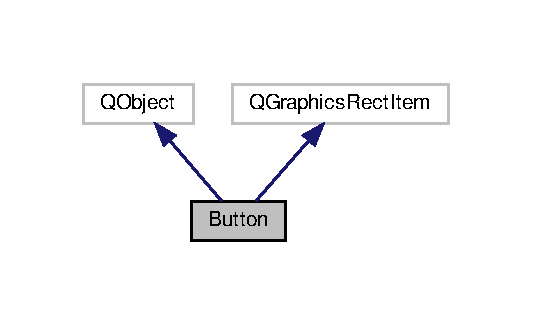
\includegraphics[width=256pt]{classButton__inherit__graph}
\end{center}
\end{figure}


Collaboration diagram for Button\+:\nopagebreak
\begin{figure}[H]
\begin{center}
\leavevmode
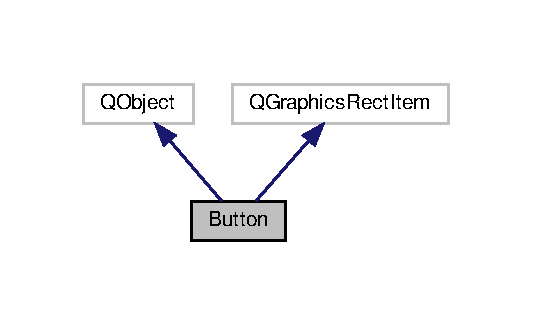
\includegraphics[width=256pt]{classButton__coll__graph}
\end{center}
\end{figure}
\subsection*{Signals}
\begin{DoxyCompactItemize}
\item 
void \hyperlink{classButton_a9e7ab4152cb1e7e3beb7f2842f32670c}{clicked} ()
\begin{DoxyCompactList}\small\item\em signal to be emitted. \end{DoxyCompactList}\end{DoxyCompactItemize}
\subsection*{Public Member Functions}
\begin{DoxyCompactItemize}
\item 
\hyperlink{classButton_a69976e5c00874a3807b642f249c1c776}{Button} (Q\+String name, Q\+Graphics\+Item $\ast$parent=N\+U\+LL)
\begin{DoxyCompactList}\small\item\em \hyperlink{classButton}{Button} constructor. \end{DoxyCompactList}\item 
void \hyperlink{classButton_a17d8eb0c904605b223bbc00c75655315}{mouse\+Press\+Event} (Q\+Graphics\+Scene\+Mouse\+Event $\ast$event)
\begin{DoxyCompactList}\small\item\em mouse press event function. \end{DoxyCompactList}\item 
void \hyperlink{classButton_a633a9684818bc5d300a622a00064f09c}{hover\+Enter\+Event} (Q\+Graphics\+Scene\+Hover\+Event $\ast$event)
\begin{DoxyCompactList}\small\item\em mouse hover event function. \end{DoxyCompactList}\item 
void \hyperlink{classButton_a1689a97690d9469ce8350d24db0d7485}{hover\+Leave\+Event} (Q\+Graphics\+Scene\+Hover\+Event $\ast$event)
\begin{DoxyCompactList}\small\item\em mouse leave event function. \end{DoxyCompactList}\end{DoxyCompactItemize}


\subsection{Detailed Description}
contains button class definition 

This class is responsible for creating a button inside a game (QT scene) 

\subsection{Constructor \& Destructor Documentation}
\mbox{\Hypertarget{classButton_a69976e5c00874a3807b642f249c1c776}\label{classButton_a69976e5c00874a3807b642f249c1c776}} 
\index{Button@{Button}!Button@{Button}}
\index{Button@{Button}!Button@{Button}}
\subsubsection{\texorpdfstring{Button()}{Button()}}
{\footnotesize\ttfamily Button\+::\+Button (\begin{DoxyParamCaption}\item[{Q\+String}]{name,  }\item[{Q\+Graphics\+Item $\ast$}]{parent = {\ttfamily NULL} }\end{DoxyParamCaption})}



\hyperlink{classButton}{Button} constructor. 

\hyperlink{classButton}{Button} constructor that takes button name as parameter. 

\subsection{Member Function Documentation}
\mbox{\Hypertarget{classButton_a9e7ab4152cb1e7e3beb7f2842f32670c}\label{classButton_a9e7ab4152cb1e7e3beb7f2842f32670c}} 
\index{Button@{Button}!clicked@{clicked}}
\index{clicked@{clicked}!Button@{Button}}
\subsubsection{\texorpdfstring{clicked}{clicked}}
{\footnotesize\ttfamily void Button\+::clicked (\begin{DoxyParamCaption}{ }\end{DoxyParamCaption})\hspace{0.3cm}{\ttfamily [signal]}}



signal to be emitted. 

signal that is emitted when the button is pressed. \mbox{\Hypertarget{classButton_a633a9684818bc5d300a622a00064f09c}\label{classButton_a633a9684818bc5d300a622a00064f09c}} 
\index{Button@{Button}!hover\+Enter\+Event@{hover\+Enter\+Event}}
\index{hover\+Enter\+Event@{hover\+Enter\+Event}!Button@{Button}}
\subsubsection{\texorpdfstring{hover\+Enter\+Event()}{hoverEnterEvent()}}
{\footnotesize\ttfamily void Button\+::hover\+Enter\+Event (\begin{DoxyParamCaption}\item[{Q\+Graphics\+Scene\+Hover\+Event $\ast$}]{event }\end{DoxyParamCaption})}



mouse hover event function. 

function that lightens up the button when the mouse is hovering over it \mbox{\Hypertarget{classButton_a1689a97690d9469ce8350d24db0d7485}\label{classButton_a1689a97690d9469ce8350d24db0d7485}} 
\index{Button@{Button}!hover\+Leave\+Event@{hover\+Leave\+Event}}
\index{hover\+Leave\+Event@{hover\+Leave\+Event}!Button@{Button}}
\subsubsection{\texorpdfstring{hover\+Leave\+Event()}{hoverLeaveEvent()}}
{\footnotesize\ttfamily void Button\+::hover\+Leave\+Event (\begin{DoxyParamCaption}\item[{Q\+Graphics\+Scene\+Hover\+Event $\ast$}]{event }\end{DoxyParamCaption})}



mouse leave event function. 

function that dims back the button when the mouse is no longer hovering over it \mbox{\Hypertarget{classButton_a17d8eb0c904605b223bbc00c75655315}\label{classButton_a17d8eb0c904605b223bbc00c75655315}} 
\index{Button@{Button}!mouse\+Press\+Event@{mouse\+Press\+Event}}
\index{mouse\+Press\+Event@{mouse\+Press\+Event}!Button@{Button}}
\subsubsection{\texorpdfstring{mouse\+Press\+Event()}{mousePressEvent()}}
{\footnotesize\ttfamily void Button\+::mouse\+Press\+Event (\begin{DoxyParamCaption}\item[{Q\+Graphics\+Scene\+Mouse\+Event $\ast$}]{event }\end{DoxyParamCaption})}



mouse press event function. 

function that sends a signal whenever the button is pressed 

The documentation for this class was generated from the following files\+:\begin{DoxyCompactItemize}
\item 
\hyperlink{button_8h}{button.\+h}\item 
button.\+cpp\end{DoxyCompactItemize}

\hypertarget{classgame1menu}{}\section{game1menu Class Reference}
\label{classgame1menu}\index{game1menu@{game1menu}}


contains game 1 menu class definition  




{\ttfamily \#include $<$game1menu.\+h$>$}



Inheritance diagram for game1menu\+:\nopagebreak
\begin{figure}[H]
\begin{center}
\leavevmode
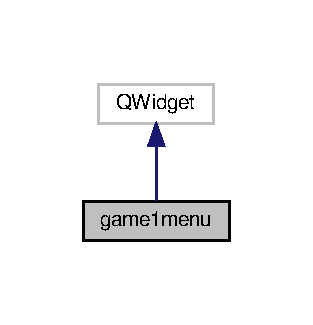
\includegraphics[width=150pt]{classgame1menu__inherit__graph}
\end{center}
\end{figure}


Collaboration diagram for game1menu\+:\nopagebreak
\begin{figure}[H]
\begin{center}
\leavevmode
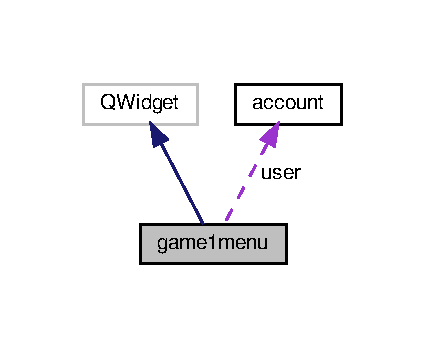
\includegraphics[width=204pt]{classgame1menu__coll__graph}
\end{center}
\end{figure}
\subsection*{Public Slots}
\begin{DoxyCompactItemize}
\item 
void \hyperlink{classgame1menu_a52cfac581c4ec8dee4b2790b773014c7}{playb} ()
\begin{DoxyCompactList}\small\item\em function to be called when play is pressed. \end{DoxyCompactList}\item 
void \hyperlink{classgame1menu_aacd43f1621af0ac39370c5f1b16868fa}{Backk} ()
\begin{DoxyCompactList}\small\item\em function to be called when back is pressed. \end{DoxyCompactList}\end{DoxyCompactItemize}
\subsection*{Public Member Functions}
\begin{DoxyCompactItemize}
\item 
\hyperlink{classgame1menu_ae63648153a4fb03068f9ee8dc3bc79dc}{game1menu} (Q\+Widget $\ast$parent=nullptr)
\begin{DoxyCompactList}\small\item\em game 1 menu constructor. \end{DoxyCompactList}\end{DoxyCompactItemize}
\subsection*{Public Attributes}
\begin{DoxyCompactItemize}
\item 
\mbox{\Hypertarget{classgame1menu_a72289ac8053ed3830cf9ea1e6655ca2c}\label{classgame1menu_a72289ac8053ed3830cf9ea1e6655ca2c}} 
Q\+Label $\ast$ \hyperlink{classgame1menu_a72289ac8053ed3830cf9ea1e6655ca2c}{title}
\begin{DoxyCompactList}\small\item\em Kill covid 19 image. \end{DoxyCompactList}\item 
\mbox{\Hypertarget{classgame1menu_aeee4023ded9672b32063b53fbe63bdea}\label{classgame1menu_aeee4023ded9672b32063b53fbe63bdea}} 
Q\+Push\+Button $\ast$ \hyperlink{classgame1menu_aeee4023ded9672b32063b53fbe63bdea}{play}
\begin{DoxyCompactList}\small\item\em Play button. \end{DoxyCompactList}\item 
\mbox{\Hypertarget{classgame1menu_a83a7c9efd9a7b4511376586768b8bcd9}\label{classgame1menu_a83a7c9efd9a7b4511376586768b8bcd9}} 
Q\+Push\+Button $\ast$ \hyperlink{classgame1menu_a83a7c9efd9a7b4511376586768b8bcd9}{back}
\begin{DoxyCompactList}\small\item\em Back button. \end{DoxyCompactList}\item 
\mbox{\Hypertarget{classgame1menu_ac95cf576945f0bb06767e31377c9e63c}\label{classgame1menu_ac95cf576945f0bb06767e31377c9e63c}} 
Q\+Label $\ast$ \hyperlink{classgame1menu_ac95cf576945f0bb06767e31377c9e63c}{l}
\begin{DoxyCompactList}\small\item\em label asking to select game level \end{DoxyCompactList}\item 
\mbox{\Hypertarget{classgame1menu_aab51ae6d3c40e2fea3e6e337a093ff0f}\label{classgame1menu_aab51ae6d3c40e2fea3e6e337a093ff0f}} 
Q\+Radio\+Button $\ast$ \hyperlink{classgame1menu_aab51ae6d3c40e2fea3e6e337a093ff0f}{lvl1}
\begin{DoxyCompactList}\small\item\em level 1 radio button \end{DoxyCompactList}\item 
\mbox{\Hypertarget{classgame1menu_a32e7765d0637c337cc195c510edde27b}\label{classgame1menu_a32e7765d0637c337cc195c510edde27b}} 
Q\+Radio\+Button $\ast$ \hyperlink{classgame1menu_a32e7765d0637c337cc195c510edde27b}{lvl2}
\begin{DoxyCompactList}\small\item\em level 2 radio button \end{DoxyCompactList}\item 
\mbox{\Hypertarget{classgame1menu_a047d717fb9fa6b3aacc15190b094195f}\label{classgame1menu_a047d717fb9fa6b3aacc15190b094195f}} 
Q\+Radio\+Button $\ast$ \hyperlink{classgame1menu_a047d717fb9fa6b3aacc15190b094195f}{lvl3}
\begin{DoxyCompactList}\small\item\em level 3 radio button \end{DoxyCompactList}\item 
\mbox{\Hypertarget{classgame1menu_a4d836229d25f2a14949d7413ea56e713}\label{classgame1menu_a4d836229d25f2a14949d7413ea56e713}} 
Q\+V\+Box\+Layout $\ast$ \hyperlink{classgame1menu_a4d836229d25f2a14949d7413ea56e713}{Vbox}
\begin{DoxyCompactList}\small\item\em Vertical box used for layout. \end{DoxyCompactList}\item 
\mbox{\Hypertarget{classgame1menu_a4d33841ad396918e93608c06b8165a12}\label{classgame1menu_a4d33841ad396918e93608c06b8165a12}} 
\hyperlink{classaccount}{account} $\ast$ \hyperlink{classgame1menu_a4d33841ad396918e93608c06b8165a12}{user}
\begin{DoxyCompactList}\small\item\em passed down user from sign in widget \end{DoxyCompactList}\end{DoxyCompactItemize}


\subsection{Detailed Description}
contains game 1 menu class definition 

This class is responsible for creating the main menu of game 1 

\subsection{Constructor \& Destructor Documentation}
\mbox{\Hypertarget{classgame1menu_ae63648153a4fb03068f9ee8dc3bc79dc}\label{classgame1menu_ae63648153a4fb03068f9ee8dc3bc79dc}} 
\index{game1menu@{game1menu}!game1menu@{game1menu}}
\index{game1menu@{game1menu}!game1menu@{game1menu}}
\subsubsection{\texorpdfstring{game1menu()}{game1menu()}}
{\footnotesize\ttfamily game1menu\+::game1menu (\begin{DoxyParamCaption}\item[{Q\+Widget $\ast$}]{parent = {\ttfamily nullptr} }\end{DoxyParamCaption})\hspace{0.3cm}{\ttfamily [explicit]}}



game 1 menu constructor. 

constructs the class and sets up the layout. also links signals to slots. 

\subsection{Member Function Documentation}
\mbox{\Hypertarget{classgame1menu_aacd43f1621af0ac39370c5f1b16868fa}\label{classgame1menu_aacd43f1621af0ac39370c5f1b16868fa}} 
\index{game1menu@{game1menu}!Backk@{Backk}}
\index{Backk@{Backk}!game1menu@{game1menu}}
\subsubsection{\texorpdfstring{Backk}{Backk}}
{\footnotesize\ttfamily void game1menu\+::\+Backk (\begin{DoxyParamCaption}{ }\end{DoxyParamCaption})\hspace{0.3cm}{\ttfamily [slot]}}



function to be called when back is pressed. 

exits the game menu and goes back to sign in widget \mbox{\Hypertarget{classgame1menu_a52cfac581c4ec8dee4b2790b773014c7}\label{classgame1menu_a52cfac581c4ec8dee4b2790b773014c7}} 
\index{game1menu@{game1menu}!playb@{playb}}
\index{playb@{playb}!game1menu@{game1menu}}
\subsubsection{\texorpdfstring{playb}{playb}}
{\footnotesize\ttfamily void game1menu\+::playb (\begin{DoxyParamCaption}{ }\end{DoxyParamCaption})\hspace{0.3cm}{\ttfamily [slot]}}



function to be called when play is pressed. 

checks which level is selected and goes to game 1 scene. each level has it\textquotesingle{}s own difficulty and music audio 

The documentation for this class was generated from the following files\+:\begin{DoxyCompactItemize}
\item 
\hyperlink{game1menu_8h}{game1menu.\+h}\item 
game1menu.\+cpp\end{DoxyCompactItemize}

\hypertarget{classgame1scene}{}\section{game1scene Class Reference}
\label{classgame1scene}\index{game1scene@{game1scene}}


contains game 1 scene class definition  




{\ttfamily \#include $<$game1scene.\+h$>$}



Inheritance diagram for game1scene\+:\nopagebreak
\begin{figure}[H]
\begin{center}
\leavevmode
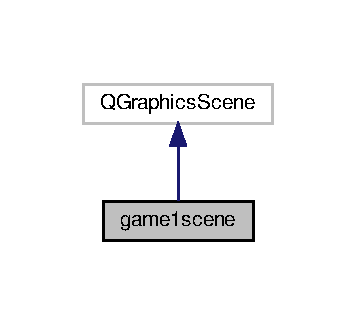
\includegraphics[width=171pt]{classgame1scene__inherit__graph}
\end{center}
\end{figure}


Collaboration diagram for game1scene\+:\nopagebreak
\begin{figure}[H]
\begin{center}
\leavevmode
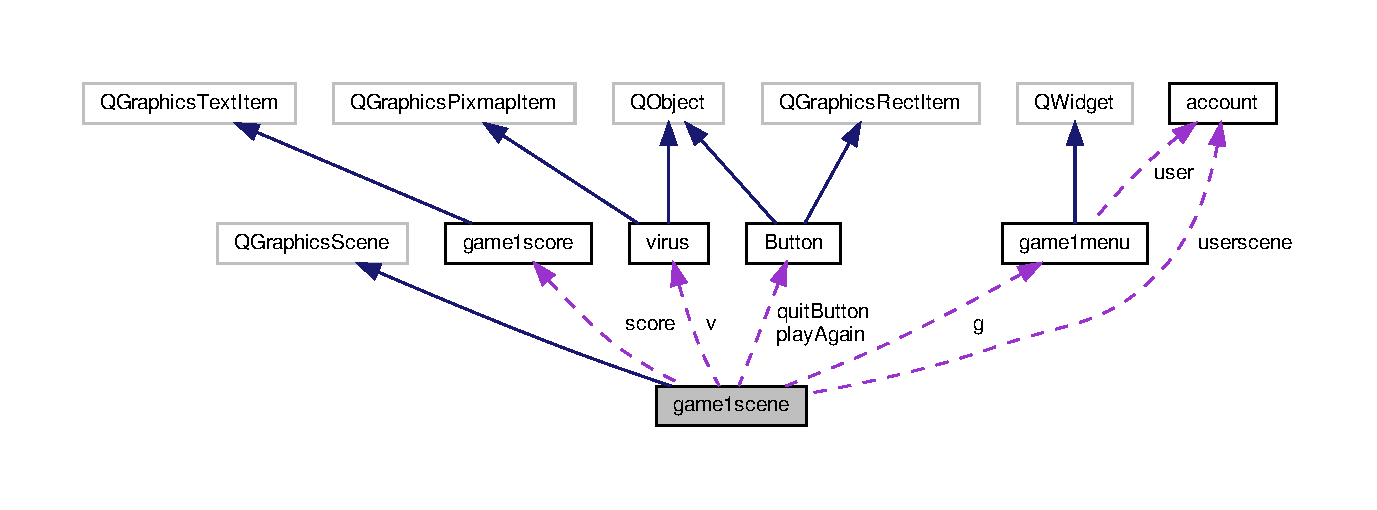
\includegraphics[width=350pt]{classgame1scene__coll__graph}
\end{center}
\end{figure}
\subsection*{Public Slots}
\begin{DoxyCompactItemize}
\item 
void \hyperlink{classgame1scene_ac85bfe270f65bee86ea75f8a0dafcd39}{create\+\_\+instance} ()
\begin{DoxyCompactList}\small\item\em creates a virus. \end{DoxyCompactList}\item 
void \hyperlink{classgame1scene_a4e66bd7b75ee140431a9ae8f9fa40000}{update\+\_\+counters} ()
\begin{DoxyCompactList}\small\item\em updates the current state of the game. \end{DoxyCompactList}\item 
void \hyperlink{classgame1scene_a62ae0fdc247d9cd0665844710b465c5c}{restart\+Game} ()
\begin{DoxyCompactList}\small\item\em Function that restarts the game. \end{DoxyCompactList}\item 
void \hyperlink{classgame1scene_a72b63628ea5dc651654db088830afd87}{quit\+Game} ()
\begin{DoxyCompactList}\small\item\em Function that quits the game. \end{DoxyCompactList}\end{DoxyCompactItemize}
\subsection*{Public Member Functions}
\begin{DoxyCompactItemize}
\item 
\hyperlink{classgame1scene_ac540834f7d119c2c89a7e17306e2a1c0}{game1scene} ()
\begin{DoxyCompactList}\small\item\em game 1 scene constructor. \end{DoxyCompactList}\item 
void \hyperlink{classgame1scene_a7ea830c4a703722bc5450f29fbfddced}{lose} ()
\begin{DoxyCompactList}\small\item\em lose function to call when you lose. \end{DoxyCompactList}\item 
void \hyperlink{classgame1scene_a760917f4ad49e991bba784f16a468f98}{win} ()
\begin{DoxyCompactList}\small\item\em win function to call when you win. \end{DoxyCompactList}\item 
void \hyperlink{classgame1scene_a730f4e696efa1ea246678e9d2a59a217}{draw\+Panel} (int x, int y, int width, int height, Q\+Color color, double opacity)
\begin{DoxyCompactList}\small\item\em function that draws a panel. \end{DoxyCompactList}\end{DoxyCompactItemize}
\subsection*{Public Attributes}
\begin{DoxyCompactItemize}
\item 
\mbox{\Hypertarget{classgame1scene_a9bb7b87c40db20bd49eea5a19e94e0f2}\label{classgame1scene_a9bb7b87c40db20bd49eea5a19e94e0f2}} 
int \hyperlink{classgame1scene_a9bb7b87c40db20bd49eea5a19e94e0f2}{i}
\begin{DoxyCompactList}\small\item\em itterator that keeps track of viruses \end{DoxyCompactList}\item 
\mbox{\Hypertarget{classgame1scene_aabc6298d95ee1230f29a8985c9a176cd}\label{classgame1scene_aabc6298d95ee1230f29a8985c9a176cd}} 
\hyperlink{classaccount}{account} $\ast$ \hyperlink{classgame1scene_aabc6298d95ee1230f29a8985c9a176cd}{userscene}
\begin{DoxyCompactList}\small\item\em user account passed down from game 1 menu \end{DoxyCompactList}\item 
\mbox{\Hypertarget{classgame1scene_aa8889d693d30062bc43c6bfa802c3baa}\label{classgame1scene_aa8889d693d30062bc43c6bfa802c3baa}} 
int \hyperlink{classgame1scene_aa8889d693d30062bc43c6bfa802c3baa}{speed}
\begin{DoxyCompactList}\small\item\em speed at which the game is running \end{DoxyCompactList}\item 
\mbox{\Hypertarget{classgame1scene_a15893603342e72e41e5d74751c58b34d}\label{classgame1scene_a15893603342e72e41e5d74751c58b34d}} 
Q\+Graphics\+View $\ast$ \hyperlink{classgame1scene_a15893603342e72e41e5d74751c58b34d}{view}
\begin{DoxyCompactList}\small\item\em view used to create the scene \end{DoxyCompactList}\item 
\mbox{\Hypertarget{classgame1scene_a4f82c0adb37a7ab736e765a4d9a87955}\label{classgame1scene_a4f82c0adb37a7ab736e765a4d9a87955}} 
Q\+Media\+Player $\ast$ \hyperlink{classgame1scene_a4f82c0adb37a7ab736e765a4d9a87955}{audio}
\begin{DoxyCompactList}\small\item\em music audio that is played during the game \end{DoxyCompactList}\item 
\mbox{\Hypertarget{classgame1scene_ade62ddcdc487fed3172557f475661207}\label{classgame1scene_ade62ddcdc487fed3172557f475661207}} 
int \hyperlink{classgame1scene_ade62ddcdc487fed3172557f475661207}{loss\+Count}
\begin{DoxyCompactList}\small\item\em stores the number of missed viruses required to lose the game \end{DoxyCompactList}\item 
\mbox{\Hypertarget{classgame1scene_a2ddd7dd6961d74ed938a9a924bf0063d}\label{classgame1scene_a2ddd7dd6961d74ed938a9a924bf0063d}} 
int \hyperlink{classgame1scene_a2ddd7dd6961d74ed938a9a924bf0063d}{score\+To\+Win}
\begin{DoxyCompactList}\small\item\em stores the score needed to win the game \end{DoxyCompactList}\item 
\mbox{\Hypertarget{classgame1scene_aab5556912872e7d31c72a911a7443244}\label{classgame1scene_aab5556912872e7d31c72a911a7443244}} 
int \hyperlink{classgame1scene_aab5556912872e7d31c72a911a7443244}{loss}
\begin{DoxyCompactList}\small\item\em keeps count of how many viruses were missed \end{DoxyCompactList}\item 
\mbox{\Hypertarget{classgame1scene_ad71ee5af83ebf44269c1985d300aa104}\label{classgame1scene_ad71ee5af83ebf44269c1985d300aa104}} 
\hyperlink{classgame1menu}{game1menu} $\ast$ \hyperlink{classgame1scene_ad71ee5af83ebf44269c1985d300aa104}{g}
\begin{DoxyCompactList}\small\item\em pointer to game 1 menu to be able to exit the game \end{DoxyCompactList}\item 
\mbox{\Hypertarget{classgame1scene_a0b20d7d61cf85c7928d181d379744219}\label{classgame1scene_a0b20d7d61cf85c7928d181d379744219}} 
Q\+File $\ast$ \hyperlink{classgame1scene_a0b20d7d61cf85c7928d181d379744219}{file}
\begin{DoxyCompactList}\small\item\em files used to read level (the txt databasse) \end{DoxyCompactList}\item 
\mbox{\Hypertarget{classgame1scene_ad5e40df47bf0f8559d640167a7137470}\label{classgame1scene_ad5e40df47bf0f8559d640167a7137470}} 
Q\+Text\+Stream $\ast$ \hyperlink{classgame1scene_ad5e40df47bf0f8559d640167a7137470}{in}
\begin{DoxyCompactList}\small\item\em Text stream used to read file. \end{DoxyCompactList}\item 
\mbox{\Hypertarget{classgame1scene_ae3928d49f36c06f044d7394ae2254b16}\label{classgame1scene_ae3928d49f36c06f044d7394ae2254b16}} 
\hyperlink{classgame1score}{game1score} $\ast$ \hyperlink{classgame1scene_ae3928d49f36c06f044d7394ae2254b16}{score}
\begin{DoxyCompactList}\small\item\em score class that keeps track of the score and displays it on the scene \end{DoxyCompactList}\item 
\mbox{\Hypertarget{classgame1scene_aceb64fd219582d9c9cfc5395155b10a5}\label{classgame1scene_aceb64fd219582d9c9cfc5395155b10a5}} 
Q\+Graphics\+Text\+Item $\ast$ \hyperlink{classgame1scene_aceb64fd219582d9c9cfc5395155b10a5}{io}
\begin{DoxyCompactList}\small\item\em text item to display either a win or a loss \end{DoxyCompactList}\item 
\mbox{\Hypertarget{classgame1scene_a35f11a42c2b6782add5943dc0b471570}\label{classgame1scene_a35f11a42c2b6782add5943dc0b471570}} 
\hyperlink{classButton}{Button} $\ast$ \hyperlink{classgame1scene_a35f11a42c2b6782add5943dc0b471570}{play\+Again}
\begin{DoxyCompactList}\small\item\em button used for Play again when the game is over \end{DoxyCompactList}\item 
\mbox{\Hypertarget{classgame1scene_a41f520712ca895f2902b17d1f1667a07}\label{classgame1scene_a41f520712ca895f2902b17d1f1667a07}} 
\hyperlink{classButton}{Button} $\ast$ \hyperlink{classgame1scene_a41f520712ca895f2902b17d1f1667a07}{quit\+Button}
\begin{DoxyCompactList}\small\item\em button used to quit the game when the game is over \end{DoxyCompactList}\item 
\mbox{\Hypertarget{classgame1scene_a5b2c75e8d9f7e2ba76089735281d432b}\label{classgame1scene_a5b2c75e8d9f7e2ba76089735281d432b}} 
Q\+Timer $\ast$ \hyperlink{classgame1scene_a5b2c75e8d9f7e2ba76089735281d432b}{inst}
\begin{DoxyCompactList}\small\item\em Timer used to call create instancce. \end{DoxyCompactList}\item 
\mbox{\Hypertarget{classgame1scene_a72a8f8545ebeb87af34de472448c8ec1}\label{classgame1scene_a72a8f8545ebeb87af34de472448c8ec1}} 
Q\+Timer $\ast$ \hyperlink{classgame1scene_a72a8f8545ebeb87af34de472448c8ec1}{count}
\begin{DoxyCompactList}\small\item\em Timer used to call update counter. \end{DoxyCompactList}\item 
\mbox{\Hypertarget{classgame1scene_a9889692b03cc597f2c5766068e81b16f}\label{classgame1scene_a9889692b03cc597f2c5766068e81b16f}} 
Q\+Graphics\+Rect\+Item $\ast$ \hyperlink{classgame1scene_a9889692b03cc597f2c5766068e81b16f}{panel}
\begin{DoxyCompactList}\small\item\em panel used to darken the screen for endgame \end{DoxyCompactList}\item 
\mbox{\Hypertarget{classgame1scene_af1eb126df2c67773e8d369465ad194ca}\label{classgame1scene_af1eb126df2c67773e8d369465ad194ca}} 
\hyperlink{classvirus}{virus} $\ast$ \hyperlink{classgame1scene_af1eb126df2c67773e8d369465ad194ca}{v} \mbox{[}40\mbox{]}
\begin{DoxyCompactList}\small\item\em array of viruses to be created \end{DoxyCompactList}\end{DoxyCompactItemize}


\subsection{Detailed Description}
contains game 1 scene class definition 

This class is responsible for creating and playing game 1 (Kill Covid-\/19) 

\subsection{Constructor \& Destructor Documentation}
\mbox{\Hypertarget{classgame1scene_ac540834f7d119c2c89a7e17306e2a1c0}\label{classgame1scene_ac540834f7d119c2c89a7e17306e2a1c0}} 
\index{game1scene@{game1scene}!game1scene@{game1scene}}
\index{game1scene@{game1scene}!game1scene@{game1scene}}
\subsubsection{\texorpdfstring{game1scene()}{game1scene()}}
{\footnotesize\ttfamily game1scene\+::game1scene (\begin{DoxyParamCaption}{ }\end{DoxyParamCaption})}



game 1 scene constructor. 

constructs game 1 scene and sets background image and initialized all elements inlucding timers and linking timers to slots. 

\subsection{Member Function Documentation}
\mbox{\Hypertarget{classgame1scene_ac85bfe270f65bee86ea75f8a0dafcd39}\label{classgame1scene_ac85bfe270f65bee86ea75f8a0dafcd39}} 
\index{game1scene@{game1scene}!create\+\_\+instance@{create\+\_\+instance}}
\index{create\+\_\+instance@{create\+\_\+instance}!game1scene@{game1scene}}
\subsubsection{\texorpdfstring{create\+\_\+instance}{create\_instance}}
{\footnotesize\ttfamily void game1scene\+::create\+\_\+instance (\begin{DoxyParamCaption}{ }\end{DoxyParamCaption})\hspace{0.3cm}{\ttfamily [slot]}}



creates a virus. 

function that creates a virus called by the timer. It checks the game level to see the size and place at which the virus should be spawned. \mbox{\Hypertarget{classgame1scene_a730f4e696efa1ea246678e9d2a59a217}\label{classgame1scene_a730f4e696efa1ea246678e9d2a59a217}} 
\index{game1scene@{game1scene}!draw\+Panel@{draw\+Panel}}
\index{draw\+Panel@{draw\+Panel}!game1scene@{game1scene}}
\subsubsection{\texorpdfstring{draw\+Panel()}{drawPanel()}}
{\footnotesize\ttfamily void game1scene\+::draw\+Panel (\begin{DoxyParamCaption}\item[{int}]{x,  }\item[{int}]{y,  }\item[{int}]{width,  }\item[{int}]{height,  }\item[{Q\+Color}]{color,  }\item[{double}]{opacity }\end{DoxyParamCaption})}



function that draws a panel. 

function that draws pannels used to create a dark panel for the end game. \mbox{\Hypertarget{classgame1scene_a7ea830c4a703722bc5450f29fbfddced}\label{classgame1scene_a7ea830c4a703722bc5450f29fbfddced}} 
\index{game1scene@{game1scene}!lose@{lose}}
\index{lose@{lose}!game1scene@{game1scene}}
\subsubsection{\texorpdfstring{lose()}{lose()}}
{\footnotesize\ttfamily void game1scene\+::lose (\begin{DoxyParamCaption}{ }\end{DoxyParamCaption})}



lose function to call when you lose. 

ends the game with a loss screen and plays a loss audio. Also writes to the account\textquotesingle{}s history the results of the game. \mbox{\Hypertarget{classgame1scene_a72b63628ea5dc651654db088830afd87}\label{classgame1scene_a72b63628ea5dc651654db088830afd87}} 
\index{game1scene@{game1scene}!quit\+Game@{quit\+Game}}
\index{quit\+Game@{quit\+Game}!game1scene@{game1scene}}
\subsubsection{\texorpdfstring{quit\+Game}{quitGame}}
{\footnotesize\ttfamily void game1scene\+::quit\+Game (\begin{DoxyParamCaption}{ }\end{DoxyParamCaption})\hspace{0.3cm}{\ttfamily [slot]}}



Function that quits the game. 

Function that quits the game when the Quit game button is pressed. goes back to game 1 menu \mbox{\Hypertarget{classgame1scene_a62ae0fdc247d9cd0665844710b465c5c}\label{classgame1scene_a62ae0fdc247d9cd0665844710b465c5c}} 
\index{game1scene@{game1scene}!restart\+Game@{restart\+Game}}
\index{restart\+Game@{restart\+Game}!game1scene@{game1scene}}
\subsubsection{\texorpdfstring{restart\+Game}{restartGame}}
{\footnotesize\ttfamily void game1scene\+::restart\+Game (\begin{DoxyParamCaption}{ }\end{DoxyParamCaption})\hspace{0.3cm}{\ttfamily [slot]}}



Function that restarts the game. 

Function that restart the game when the Restart button is pressed. \mbox{\Hypertarget{classgame1scene_a4e66bd7b75ee140431a9ae8f9fa40000}\label{classgame1scene_a4e66bd7b75ee140431a9ae8f9fa40000}} 
\index{game1scene@{game1scene}!update\+\_\+counters@{update\+\_\+counters}}
\index{update\+\_\+counters@{update\+\_\+counters}!game1scene@{game1scene}}
\subsubsection{\texorpdfstring{update\+\_\+counters}{update\_counters}}
{\footnotesize\ttfamily void game1scene\+::update\+\_\+counters (\begin{DoxyParamCaption}{ }\end{DoxyParamCaption})\hspace{0.3cm}{\ttfamily [slot]}}



updates the current state of the game. 

updates the current state of the game by updating the score, counts and checks for win/loss conditions. \mbox{\Hypertarget{classgame1scene_a760917f4ad49e991bba784f16a468f98}\label{classgame1scene_a760917f4ad49e991bba784f16a468f98}} 
\index{game1scene@{game1scene}!win@{win}}
\index{win@{win}!game1scene@{game1scene}}
\subsubsection{\texorpdfstring{win()}{win()}}
{\footnotesize\ttfamily void game1scene\+::win (\begin{DoxyParamCaption}{ }\end{DoxyParamCaption})}



win function to call when you win. 

ends the game with a win screen and plays a victory sound. Also writes to the account\textquotesingle{}s history the results of the game. 

The documentation for this class was generated from the following files\+:\begin{DoxyCompactItemize}
\item 
\hyperlink{game1scene_8h}{game1scene.\+h}\item 
game1scene.\+cpp\end{DoxyCompactItemize}

\hypertarget{classgame1score}{}\section{game1score Class Reference}
\label{classgame1score}\index{game1score@{game1score}}


contains game 1 score class definition  




{\ttfamily \#include $<$game1score.\+h$>$}



Inheritance diagram for game1score\+:\nopagebreak
\begin{figure}[H]
\begin{center}
\leavevmode
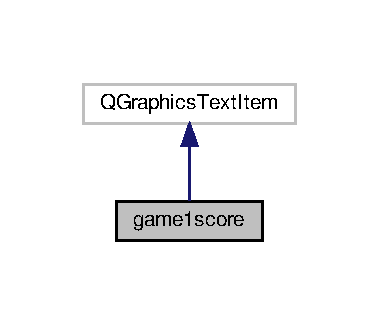
\includegraphics[width=182pt]{classgame1score__inherit__graph}
\end{center}
\end{figure}


Collaboration diagram for game1score\+:\nopagebreak
\begin{figure}[H]
\begin{center}
\leavevmode
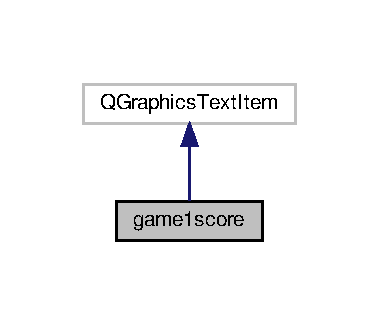
\includegraphics[width=182pt]{classgame1score__coll__graph}
\end{center}
\end{figure}
\subsection*{Public Member Functions}
\begin{DoxyCompactItemize}
\item 
\hyperlink{classgame1score_ab80521983d8a77a466dd7d7253fcd647}{game1score} (Q\+Graphics\+Item $\ast$parent=nullptr)
\begin{DoxyCompactList}\small\item\em game 1 score constructor. \end{DoxyCompactList}\item 
void \hyperlink{classgame1score_a8e7db583a40c885711eae334d4c695cd}{si} ()
\begin{DoxyCompactList}\small\item\em updates score when small virus is killed. \end{DoxyCompactList}\item 
void \hyperlink{classgame1score_a7b29421704c3766a8535fa878b3036d9}{mi} ()
\begin{DoxyCompactList}\small\item\em updates score when medium virus is killed. \end{DoxyCompactList}\item 
void \hyperlink{classgame1score_aa2aecd005fd86671e508a3b91f4251b6}{bi} ()
\begin{DoxyCompactList}\small\item\em updates score when big virus is killed. \end{DoxyCompactList}\end{DoxyCompactItemize}
\subsection*{Public Attributes}
\begin{DoxyCompactItemize}
\item 
\mbox{\Hypertarget{classgame1score_a5cdaac95a04c8036bf56c01f8fa3099e}\label{classgame1score_a5cdaac95a04c8036bf56c01f8fa3099e}} 
int \hyperlink{classgame1score_a5cdaac95a04c8036bf56c01f8fa3099e}{scount}
\begin{DoxyCompactList}\small\item\em stores small count \end{DoxyCompactList}\item 
\mbox{\Hypertarget{classgame1score_ab4ad7f19068b4719593cc7b4ee7dbd06}\label{classgame1score_ab4ad7f19068b4719593cc7b4ee7dbd06}} 
int \hyperlink{classgame1score_ab4ad7f19068b4719593cc7b4ee7dbd06}{mcount}
\begin{DoxyCompactList}\small\item\em stores medium count \end{DoxyCompactList}\item 
\mbox{\Hypertarget{classgame1score_a1396fb2d6d045ca1726b9b34e130ec8f}\label{classgame1score_a1396fb2d6d045ca1726b9b34e130ec8f}} 
int \hyperlink{classgame1score_a1396fb2d6d045ca1726b9b34e130ec8f}{bcount}
\begin{DoxyCompactList}\small\item\em stores big count \end{DoxyCompactList}\item 
\mbox{\Hypertarget{classgame1score_af8f924e5fbe567b2583583d2d95550d7}\label{classgame1score_af8f924e5fbe567b2583583d2d95550d7}} 
int \hyperlink{classgame1score_af8f924e5fbe567b2583583d2d95550d7}{score}
\begin{DoxyCompactList}\small\item\em stores total game score \end{DoxyCompactList}\item 
\mbox{\Hypertarget{classgame1score_a2fdce0ba179a04bfbbd5f296040bb2f7}\label{classgame1score_a2fdce0ba179a04bfbbd5f296040bb2f7}} 
int \hyperlink{classgame1score_a2fdce0ba179a04bfbbd5f296040bb2f7}{sum}
\begin{DoxyCompactList}\small\item\em stores the sum of scount, mcount and bcount \end{DoxyCompactList}\item 
\mbox{\Hypertarget{classgame1score_aee8bbcda0471c31f20a0beea6d7c0c17}\label{classgame1score_aee8bbcda0471c31f20a0beea6d7c0c17}} 
Q\+String \hyperlink{classgame1score_aee8bbcda0471c31f20a0beea6d7c0c17}{text}
\begin{DoxyCompactList}\small\item\em text to be displayed on screen as score \end{DoxyCompactList}\end{DoxyCompactItemize}


\subsection{Detailed Description}
contains game 1 score class definition 

This class is responsible for keeping track of the score and displaying it in game 1 

\subsection{Constructor \& Destructor Documentation}
\mbox{\Hypertarget{classgame1score_ab80521983d8a77a466dd7d7253fcd647}\label{classgame1score_ab80521983d8a77a466dd7d7253fcd647}} 
\index{game1score@{game1score}!game1score@{game1score}}
\index{game1score@{game1score}!game1score@{game1score}}
\subsubsection{\texorpdfstring{game1score()}{game1score()}}
{\footnotesize\ttfamily game1score\+::game1score (\begin{DoxyParamCaption}\item[{Q\+Graphics\+Item $\ast$}]{parent = {\ttfamily nullptr} }\end{DoxyParamCaption})\hspace{0.3cm}{\ttfamily [explicit]}}



game 1 score constructor. 

constructs the class and sets all scores to 0. additionally sets the base text to be displayed in game 1 scene. 

\subsection{Member Function Documentation}
\mbox{\Hypertarget{classgame1score_aa2aecd005fd86671e508a3b91f4251b6}\label{classgame1score_aa2aecd005fd86671e508a3b91f4251b6}} 
\index{game1score@{game1score}!bi@{bi}}
\index{bi@{bi}!game1score@{game1score}}
\subsubsection{\texorpdfstring{bi()}{bi()}}
{\footnotesize\ttfamily void game1score\+::bi (\begin{DoxyParamCaption}{ }\end{DoxyParamCaption})}



updates score when big virus is killed. 

updates score when big virus is killed by incrementing big count by 1 and score by 7. \mbox{\Hypertarget{classgame1score_a7b29421704c3766a8535fa878b3036d9}\label{classgame1score_a7b29421704c3766a8535fa878b3036d9}} 
\index{game1score@{game1score}!mi@{mi}}
\index{mi@{mi}!game1score@{game1score}}
\subsubsection{\texorpdfstring{mi()}{mi()}}
{\footnotesize\ttfamily void game1score\+::mi (\begin{DoxyParamCaption}{ }\end{DoxyParamCaption})}



updates score when medium virus is killed. 

updates score when medium virus is killed by incrementing medium count by 1 and score by 5. \mbox{\Hypertarget{classgame1score_a8e7db583a40c885711eae334d4c695cd}\label{classgame1score_a8e7db583a40c885711eae334d4c695cd}} 
\index{game1score@{game1score}!si@{si}}
\index{si@{si}!game1score@{game1score}}
\subsubsection{\texorpdfstring{si()}{si()}}
{\footnotesize\ttfamily void game1score\+::si (\begin{DoxyParamCaption}{ }\end{DoxyParamCaption})}



updates score when small virus is killed. 

updates score when small virus is killed by incrementing small count by 1 and score by 3. 

The documentation for this class was generated from the following files\+:\begin{DoxyCompactItemize}
\item 
game1score.\+h\item 
game1score.\+cpp\end{DoxyCompactItemize}

\hypertarget{classgame2menu}{}\section{game2menu Class Reference}
\label{classgame2menu}\index{game2menu@{game2menu}}


contains game 2 menu class definition  




{\ttfamily \#include $<$game2menu.\+h$>$}



Inheritance diagram for game2menu\+:\nopagebreak
\begin{figure}[H]
\begin{center}
\leavevmode
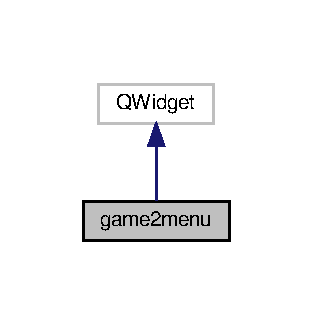
\includegraphics[width=150pt]{classgame2menu__inherit__graph}
\end{center}
\end{figure}


Collaboration diagram for game2menu\+:\nopagebreak
\begin{figure}[H]
\begin{center}
\leavevmode
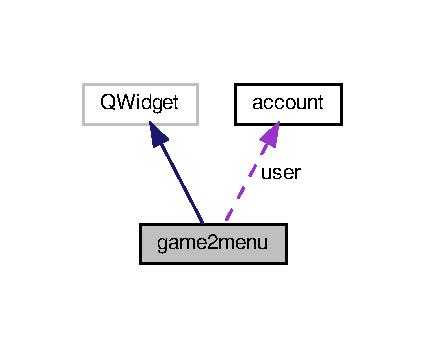
\includegraphics[width=204pt]{classgame2menu__coll__graph}
\end{center}
\end{figure}
\subsection*{Public Slots}
\begin{DoxyCompactItemize}
\item 
void \hyperlink{classgame2menu_a329e5585c0d5c6af4c4f4011efa6878f}{playb} ()
\begin{DoxyCompactList}\small\item\em function to be called when play is pressed. \end{DoxyCompactList}\item 
void \hyperlink{classgame2menu_a095e776799d92c9d6cb05aa49b63472a}{Backk} ()
\begin{DoxyCompactList}\small\item\em function to be called when back is pressed. \end{DoxyCompactList}\end{DoxyCompactItemize}
\subsection*{Public Member Functions}
\begin{DoxyCompactItemize}
\item 
\hyperlink{classgame2menu_adbca99dd8b328bab30bb1a5f198cb849}{game2menu} (Q\+Widget $\ast$parent=nullptr)
\begin{DoxyCompactList}\small\item\em game 1 menu constructor. \end{DoxyCompactList}\end{DoxyCompactItemize}
\subsection*{Public Attributes}
\begin{DoxyCompactItemize}
\item 
\mbox{\Hypertarget{classgame2menu_ad425f6fa5fc38be976fde532f173b202}\label{classgame2menu_ad425f6fa5fc38be976fde532f173b202}} 
Q\+Label $\ast$ \hyperlink{classgame2menu_ad425f6fa5fc38be976fde532f173b202}{title}
\begin{DoxyCompactList}\small\item\em Othello title image. \end{DoxyCompactList}\item 
\mbox{\Hypertarget{classgame2menu_a3d3484e23586e4219eeefabbc0203afb}\label{classgame2menu_a3d3484e23586e4219eeefabbc0203afb}} 
Q\+Push\+Button $\ast$ \hyperlink{classgame2menu_a3d3484e23586e4219eeefabbc0203afb}{play}
\begin{DoxyCompactList}\small\item\em Play button. \end{DoxyCompactList}\item 
\mbox{\Hypertarget{classgame2menu_a6015c161e82f886cc9193f397b03a24d}\label{classgame2menu_a6015c161e82f886cc9193f397b03a24d}} 
Q\+Push\+Button $\ast$ \hyperlink{classgame2menu_a6015c161e82f886cc9193f397b03a24d}{back}
\begin{DoxyCompactList}\small\item\em Back button. \end{DoxyCompactList}\item 
\mbox{\Hypertarget{classgame2menu_a2f79ea6f000654ef0092f4d4b9364382}\label{classgame2menu_a2f79ea6f000654ef0092f4d4b9364382}} 
Q\+V\+Box\+Layout $\ast$ \hyperlink{classgame2menu_a2f79ea6f000654ef0092f4d4b9364382}{Vbox}
\begin{DoxyCompactList}\small\item\em Vertical box used for layout. \end{DoxyCompactList}\item 
\mbox{\Hypertarget{classgame2menu_a081baa426df4a4a194314316e1451dc3}\label{classgame2menu_a081baa426df4a4a194314316e1451dc3}} 
\hyperlink{classaccount}{account} $\ast$ \hyperlink{classgame2menu_a081baa426df4a4a194314316e1451dc3}{user}
\begin{DoxyCompactList}\small\item\em passed down user from sign in widget \end{DoxyCompactList}\end{DoxyCompactItemize}


\subsection{Detailed Description}
contains game 2 menu class definition 

This class is responsible for creating the main menu of game 2 

\subsection{Constructor \& Destructor Documentation}
\mbox{\Hypertarget{classgame2menu_adbca99dd8b328bab30bb1a5f198cb849}\label{classgame2menu_adbca99dd8b328bab30bb1a5f198cb849}} 
\index{game2menu@{game2menu}!game2menu@{game2menu}}
\index{game2menu@{game2menu}!game2menu@{game2menu}}
\subsubsection{\texorpdfstring{game2menu()}{game2menu()}}
{\footnotesize\ttfamily game2menu\+::game2menu (\begin{DoxyParamCaption}\item[{Q\+Widget $\ast$}]{parent = {\ttfamily nullptr} }\end{DoxyParamCaption})\hspace{0.3cm}{\ttfamily [explicit]}}



game 1 menu constructor. 

constructs the class and sets up the layout. also links signals to slots. 

\subsection{Member Function Documentation}
\mbox{\Hypertarget{classgame2menu_a095e776799d92c9d6cb05aa49b63472a}\label{classgame2menu_a095e776799d92c9d6cb05aa49b63472a}} 
\index{game2menu@{game2menu}!Backk@{Backk}}
\index{Backk@{Backk}!game2menu@{game2menu}}
\subsubsection{\texorpdfstring{Backk}{Backk}}
{\footnotesize\ttfamily void game2menu\+::\+Backk (\begin{DoxyParamCaption}{ }\end{DoxyParamCaption})\hspace{0.3cm}{\ttfamily [slot]}}



function to be called when back is pressed. 

exits the game menu and goes back to sign in widget \mbox{\Hypertarget{classgame2menu_a329e5585c0d5c6af4c4f4011efa6878f}\label{classgame2menu_a329e5585c0d5c6af4c4f4011efa6878f}} 
\index{game2menu@{game2menu}!playb@{playb}}
\index{playb@{playb}!game2menu@{game2menu}}
\subsubsection{\texorpdfstring{playb}{playb}}
{\footnotesize\ttfamily void game2menu\+::playb (\begin{DoxyParamCaption}{ }\end{DoxyParamCaption})\hspace{0.3cm}{\ttfamily [slot]}}



function to be called when play is pressed. 

checks goes to game 2 scene. 

The documentation for this class was generated from the following files\+:\begin{DoxyCompactItemize}
\item 
game2menu.\+h\item 
game2menu.\+cpp\end{DoxyCompactItemize}

\hypertarget{classgame2scene}{}\section{game2scene Class Reference}
\label{classgame2scene}\index{game2scene@{game2scene}}


contains game 2 scene class definition  




{\ttfamily \#include $<$game2scene.\+h$>$}



Inheritance diagram for game2scene\+:\nopagebreak
\begin{figure}[H]
\begin{center}
\leavevmode
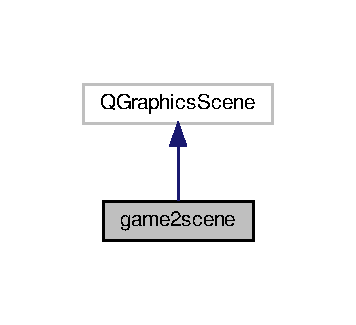
\includegraphics[width=171pt]{classgame2scene__inherit__graph}
\end{center}
\end{figure}


Collaboration diagram for game2scene\+:\nopagebreak
\begin{figure}[H]
\begin{center}
\leavevmode
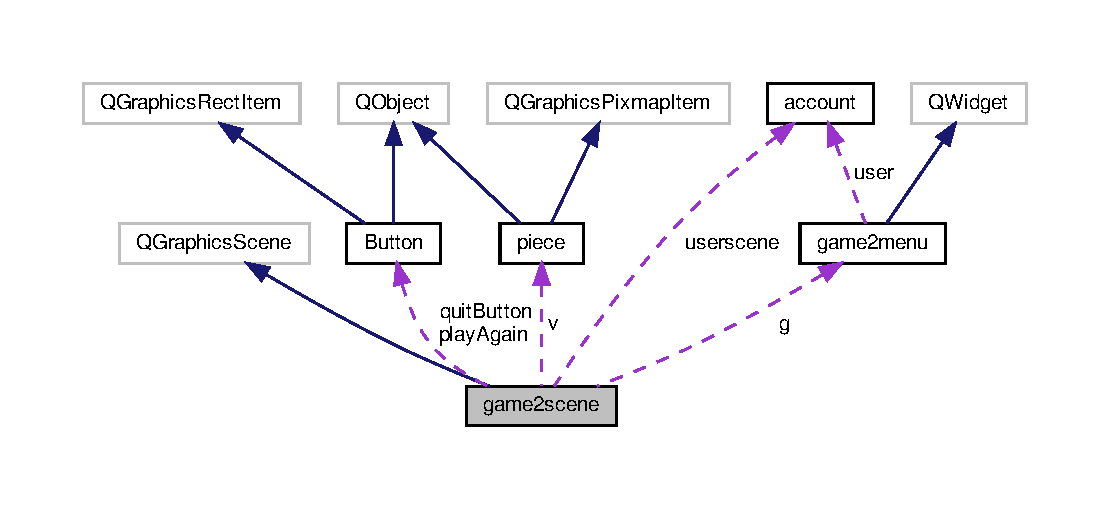
\includegraphics[width=350pt]{classgame2scene__coll__graph}
\end{center}
\end{figure}
\subsection*{Public Slots}
\begin{DoxyCompactItemize}
\item 
void \hyperlink{classgame2scene_a9ff06546f203c57909aaeb36063fc206}{check\+Fresh} ()
\begin{DoxyCompactList}\small\item\em Function that is called when a signal is emitted from any piece. \end{DoxyCompactList}\item 
void \hyperlink{classgame2scene_a8b3ee51f004d034df994bd602a31ec5b}{restart\+Game} ()
\begin{DoxyCompactList}\small\item\em Function that restarts the game. \end{DoxyCompactList}\item 
void \hyperlink{classgame2scene_ab8f07d5d6dacd32de1ff442ee29f45d3}{quit\+Game} ()
\begin{DoxyCompactList}\small\item\em Function that quits the game. \end{DoxyCompactList}\end{DoxyCompactItemize}
\subsection*{Public Member Functions}
\begin{DoxyCompactItemize}
\item 
\hyperlink{classgame2scene_aa3642161921dd08a8fa5c83e94c2ffe0}{game2scene} ()
\begin{DoxyCompactList}\small\item\em game 2 scene constructor. \end{DoxyCompactList}\item 
void \hyperlink{classgame2scene_a507687b5f74b925022c7a43749cf6607}{draw\+Panel} (int x, int y, int width, int height, Q\+Color color, double opacity)
\begin{DoxyCompactList}\small\item\em function that draws a panel. \end{DoxyCompactList}\item 
void \hyperlink{classgame2scene_a62c522d6732ff2a4889ba59ccc74f0dc}{outflank} (int i, int j)
\begin{DoxyCompactList}\small\item\em Outflank function. \end{DoxyCompactList}\item 
bool \hyperlink{classgame2scene_ae58d542526a191cf327675b83694f4ec}{checklegal} ()
\begin{DoxyCompactList}\small\item\em function that checks which pieces should be valid. \end{DoxyCompactList}\item 
void \hyperlink{classgame2scene_a6ce6a4eaa445f93d88e48d2bf06b0a13}{end} ()
\begin{DoxyCompactList}\small\item\em end game function. \end{DoxyCompactList}\end{DoxyCompactItemize}
\subsection*{Public Attributes}
\begin{DoxyCompactItemize}
\item 
\mbox{\Hypertarget{classgame2scene_a63a51aeeb0e5d6afcc135d6e6b3673ed}\label{classgame2scene_a63a51aeeb0e5d6afcc135d6e6b3673ed}} 
\hyperlink{classaccount}{account} $\ast$ \hyperlink{classgame2scene_a63a51aeeb0e5d6afcc135d6e6b3673ed}{userscene}
\begin{DoxyCompactList}\small\item\em user account passed down from game 1 menu \end{DoxyCompactList}\item 
\mbox{\Hypertarget{classgame2scene_aa97a0971c7aa75079ec09827ffde1d25}\label{classgame2scene_aa97a0971c7aa75079ec09827ffde1d25}} 
Q\+Graphics\+View $\ast$ \hyperlink{classgame2scene_aa97a0971c7aa75079ec09827ffde1d25}{view}
\begin{DoxyCompactList}\small\item\em view used to create the scene \end{DoxyCompactList}\item 
\mbox{\Hypertarget{classgame2scene_a9e5eb644437aa33b94e9aadd0364aad7}\label{classgame2scene_a9e5eb644437aa33b94e9aadd0364aad7}} 
\hyperlink{classpiece}{piece} $\ast$ \hyperlink{classgame2scene_a9e5eb644437aa33b94e9aadd0364aad7}{v} \mbox{[}8\mbox{]}\mbox{[}8\mbox{]}
\begin{DoxyCompactList}\small\item\em Double array containing all 64 pieces of the game. \end{DoxyCompactList}\item 
\mbox{\Hypertarget{classgame2scene_ad931a8f0808eed7e85f974669a303767}\label{classgame2scene_ad931a8f0808eed7e85f974669a303767}} 
Q\+Media\+Player $\ast$ \hyperlink{classgame2scene_ad931a8f0808eed7e85f974669a303767}{au}
\begin{DoxyCompactList}\small\item\em adio player used to play different sounds \end{DoxyCompactList}\item 
\mbox{\Hypertarget{classgame2scene_a1c4812d12e0e31e150d2dc1d6fc8b672}\label{classgame2scene_a1c4812d12e0e31e150d2dc1d6fc8b672}} 
Q\+Graphics\+Rect\+Item $\ast$ \hyperlink{classgame2scene_a1c4812d12e0e31e150d2dc1d6fc8b672}{panel}
\begin{DoxyCompactList}\small\item\em panel used to darken the screen for endgame \end{DoxyCompactList}\item 
\mbox{\Hypertarget{classgame2scene_a99c8aa963d23ccffbcc4f3fca4b2fb2e}\label{classgame2scene_a99c8aa963d23ccffbcc4f3fca4b2fb2e}} 
Q\+Graphics\+Text\+Item $\ast$ \hyperlink{classgame2scene_a99c8aa963d23ccffbcc4f3fca4b2fb2e}{io}
\begin{DoxyCompactList}\small\item\em text item to display who won and the score \end{DoxyCompactList}\item 
\mbox{\Hypertarget{classgame2scene_a791537ed5b1fb8d2a007dee9ba6916d4}\label{classgame2scene_a791537ed5b1fb8d2a007dee9ba6916d4}} 
\hyperlink{classgame2menu}{game2menu} $\ast$ \hyperlink{classgame2scene_a791537ed5b1fb8d2a007dee9ba6916d4}{g}
\begin{DoxyCompactList}\small\item\em pointer to game 2 menu to be able to exit the game \end{DoxyCompactList}\item 
\mbox{\Hypertarget{classgame2scene_ad42a753ce56a92b1963258a64b6a29d3}\label{classgame2scene_ad42a753ce56a92b1963258a64b6a29d3}} 
\hyperlink{classButton}{Button} $\ast$ \hyperlink{classgame2scene_ad42a753ce56a92b1963258a64b6a29d3}{play\+Again}
\begin{DoxyCompactList}\small\item\em button used for Play again when the game is over \end{DoxyCompactList}\item 
\mbox{\Hypertarget{classgame2scene_a87b11f6fc01d8073e9421d4b39aa2ddb}\label{classgame2scene_a87b11f6fc01d8073e9421d4b39aa2ddb}} 
\hyperlink{classButton}{Button} $\ast$ \hyperlink{classgame2scene_a87b11f6fc01d8073e9421d4b39aa2ddb}{quit\+Button}
\begin{DoxyCompactList}\small\item\em button used to quit the game when the game is over \end{DoxyCompactList}\end{DoxyCompactItemize}


\subsection{Detailed Description}
contains game 2 scene class definition 

This class is responsible for creating and playing game 2 (othello or reversi) 

\subsection{Constructor \& Destructor Documentation}
\mbox{\Hypertarget{classgame2scene_aa3642161921dd08a8fa5c83e94c2ffe0}\label{classgame2scene_aa3642161921dd08a8fa5c83e94c2ffe0}} 
\index{game2scene@{game2scene}!game2scene@{game2scene}}
\index{game2scene@{game2scene}!game2scene@{game2scene}}
\subsubsection{\texorpdfstring{game2scene()}{game2scene()}}
{\footnotesize\ttfamily game2scene\+::game2scene (\begin{DoxyParamCaption}{ }\end{DoxyParamCaption})}



game 2 scene constructor. 

constructs game 2 scene and sets background image and initialized all elements inlucding all 64 pieces links their signals to the correct slots. 

\subsection{Member Function Documentation}
\mbox{\Hypertarget{classgame2scene_a9ff06546f203c57909aaeb36063fc206}\label{classgame2scene_a9ff06546f203c57909aaeb36063fc206}} 
\index{game2scene@{game2scene}!check\+Fresh@{check\+Fresh}}
\index{check\+Fresh@{check\+Fresh}!game2scene@{game2scene}}
\subsubsection{\texorpdfstring{check\+Fresh}{checkFresh}}
{\footnotesize\ttfamily void game2scene\+::check\+Fresh (\begin{DoxyParamCaption}{ }\end{DoxyParamCaption})\hspace{0.3cm}{\ttfamily [slot]}}



Function that is called when a signal is emitted from any piece. 

This function is called whenever a signal is emitted from any piece, It searches for the fresh or newest piece placed on the board and calls the function outflank. \mbox{\Hypertarget{classgame2scene_ae58d542526a191cf327675b83694f4ec}\label{classgame2scene_ae58d542526a191cf327675b83694f4ec}} 
\index{game2scene@{game2scene}!checklegal@{checklegal}}
\index{checklegal@{checklegal}!game2scene@{game2scene}}
\subsubsection{\texorpdfstring{checklegal()}{checklegal()}}
{\footnotesize\ttfamily bool game2scene\+::checklegal (\begin{DoxyParamCaption}{ }\end{DoxyParamCaption})}



function that checks which pieces should be valid. 

this boolean function checks all pieces on the board from all directions to see if they are outflankable. if a piece is outflankable this piece is set to valid. this function returns false if no valid piece is found and thus does not switch turns else it returns true. \mbox{\Hypertarget{classgame2scene_a507687b5f74b925022c7a43749cf6607}\label{classgame2scene_a507687b5f74b925022c7a43749cf6607}} 
\index{game2scene@{game2scene}!draw\+Panel@{draw\+Panel}}
\index{draw\+Panel@{draw\+Panel}!game2scene@{game2scene}}
\subsubsection{\texorpdfstring{draw\+Panel()}{drawPanel()}}
{\footnotesize\ttfamily void game2scene\+::draw\+Panel (\begin{DoxyParamCaption}\item[{int}]{x,  }\item[{int}]{y,  }\item[{int}]{width,  }\item[{int}]{height,  }\item[{Q\+Color}]{color,  }\item[{double}]{opacity }\end{DoxyParamCaption})}



function that draws a panel. 

function that draws pannels used to create a dark panel for the end game. \mbox{\Hypertarget{classgame2scene_a6ce6a4eaa445f93d88e48d2bf06b0a13}\label{classgame2scene_a6ce6a4eaa445f93d88e48d2bf06b0a13}} 
\index{game2scene@{game2scene}!end@{end}}
\index{end@{end}!game2scene@{game2scene}}
\subsubsection{\texorpdfstring{end()}{end()}}
{\footnotesize\ttfamily void game2scene\+::end (\begin{DoxyParamCaption}{ }\end{DoxyParamCaption})}



end game function. 

when the game is over, this function checks who won, display the end game scene on the view and plays a victory sound. \mbox{\Hypertarget{classgame2scene_a62c522d6732ff2a4889ba59ccc74f0dc}\label{classgame2scene_a62c522d6732ff2a4889ba59ccc74f0dc}} 
\index{game2scene@{game2scene}!outflank@{outflank}}
\index{outflank@{outflank}!game2scene@{game2scene}}
\subsubsection{\texorpdfstring{outflank()}{outflank()}}
{\footnotesize\ttfamily void game2scene\+::outflank (\begin{DoxyParamCaption}\item[{int}]{i,  }\item[{int}]{j }\end{DoxyParamCaption})}



Outflank function. 

this function takes the location of a piece and checks all 8 directions around it if it can outflank the enemy pieces and outflanks them. At the end, the function checklegal is called and the turn is changed. \mbox{\Hypertarget{classgame2scene_ab8f07d5d6dacd32de1ff442ee29f45d3}\label{classgame2scene_ab8f07d5d6dacd32de1ff442ee29f45d3}} 
\index{game2scene@{game2scene}!quit\+Game@{quit\+Game}}
\index{quit\+Game@{quit\+Game}!game2scene@{game2scene}}
\subsubsection{\texorpdfstring{quit\+Game}{quitGame}}
{\footnotesize\ttfamily void game2scene\+::quit\+Game (\begin{DoxyParamCaption}{ }\end{DoxyParamCaption})\hspace{0.3cm}{\ttfamily [slot]}}



Function that quits the game. 

Function that quits the game when the Quit game button is pressed. goes back to game 2 menu \mbox{\Hypertarget{classgame2scene_a8b3ee51f004d034df994bd602a31ec5b}\label{classgame2scene_a8b3ee51f004d034df994bd602a31ec5b}} 
\index{game2scene@{game2scene}!restart\+Game@{restart\+Game}}
\index{restart\+Game@{restart\+Game}!game2scene@{game2scene}}
\subsubsection{\texorpdfstring{restart\+Game}{restartGame}}
{\footnotesize\ttfamily void game2scene\+::restart\+Game (\begin{DoxyParamCaption}{ }\end{DoxyParamCaption})\hspace{0.3cm}{\ttfamily [slot]}}



Function that restarts the game. 

Function that restart the game when the Restart button is pressed. 

The documentation for this class was generated from the following files\+:\begin{DoxyCompactItemize}
\item 
\hyperlink{game2scene_8h}{game2scene.\+h}\item 
game2scene.\+cpp\end{DoxyCompactItemize}

\hypertarget{classhistorywidget}{}\section{historywidget Class Reference}
\label{classhistorywidget}\index{historywidget@{historywidget}}


contains history widget class defintion  




{\ttfamily \#include $<$historywidget.\+h$>$}



Inheritance diagram for historywidget\+:\nopagebreak
\begin{figure}[H]
\begin{center}
\leavevmode
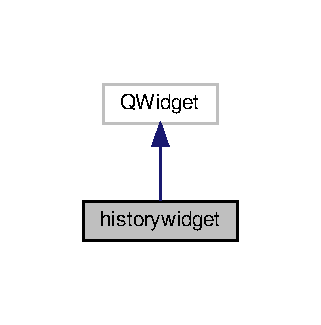
\includegraphics[width=154pt]{classhistorywidget__inherit__graph}
\end{center}
\end{figure}


Collaboration diagram for historywidget\+:\nopagebreak
\begin{figure}[H]
\begin{center}
\leavevmode
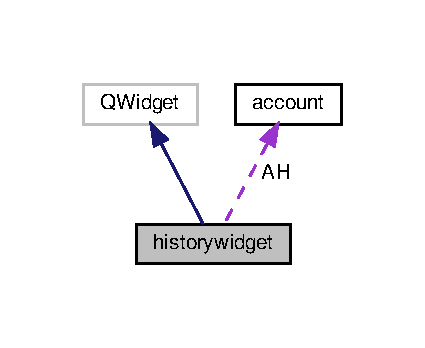
\includegraphics[width=204pt]{classhistorywidget__coll__graph}
\end{center}
\end{figure}
\subsection*{Public Slots}
\begin{DoxyCompactItemize}
\item 
void \hyperlink{classhistorywidget_a19aa3f9d16ac28a32b31b340623b0611}{Back1} ()
\begin{DoxyCompactList}\small\item\em back slot \end{DoxyCompactList}\end{DoxyCompactItemize}
\subsection*{Public Member Functions}
\begin{DoxyCompactItemize}
\item 
\hyperlink{classhistorywidget_ac21cb2c9cdecd91ac572d8fc8ba50708}{historywidget} (Q\+Widget $\ast$parent=nullptr)
\begin{DoxyCompactList}\small\item\em history widget constructor \end{DoxyCompactList}\item 
void \hyperlink{classhistorywidget_aa2edafd200341f9273bc3c8c4930902e}{get\+History} ()
\begin{DoxyCompactList}\small\item\em Get history function. \end{DoxyCompactList}\end{DoxyCompactItemize}
\subsection*{Public Attributes}
\begin{DoxyCompactItemize}
\item 
\mbox{\Hypertarget{classhistorywidget_a9d630c4651725438d7161588bd084248}\label{classhistorywidget_a9d630c4651725438d7161588bd084248}} 
\hyperlink{classaccount}{account} $\ast$ \hyperlink{classhistorywidget_a9d630c4651725438d7161588bd084248}{AH}
\begin{DoxyCompactList}\small\item\em account \end{DoxyCompactList}\item 
\mbox{\Hypertarget{classhistorywidget_aa03cf30ef4ba1cf78f4e903d981d9783}\label{classhistorywidget_aa03cf30ef4ba1cf78f4e903d981d9783}} 
Q\+Push\+Button $\ast$ \hyperlink{classhistorywidget_aa03cf30ef4ba1cf78f4e903d981d9783}{back}
\begin{DoxyCompactList}\small\item\em back button \end{DoxyCompactList}\item 
\mbox{\Hypertarget{classhistorywidget_a2f81897b41709e0218730acb285e60ea}\label{classhistorywidget_a2f81897b41709e0218730acb285e60ea}} 
Q\+V\+Box\+Layout $\ast$ \hyperlink{classhistorywidget_a2f81897b41709e0218730acb285e60ea}{V\+Box}
\begin{DoxyCompactList}\small\item\em vertical box layout \end{DoxyCompactList}\end{DoxyCompactItemize}


\subsection{Detailed Description}
contains history widget class defintion 

This class is responsible for constructing the history widget 

\subsection{Constructor \& Destructor Documentation}
\mbox{\Hypertarget{classhistorywidget_ac21cb2c9cdecd91ac572d8fc8ba50708}\label{classhistorywidget_ac21cb2c9cdecd91ac572d8fc8ba50708}} 
\index{historywidget@{historywidget}!historywidget@{historywidget}}
\index{historywidget@{historywidget}!historywidget@{historywidget}}
\subsubsection{\texorpdfstring{historywidget()}{historywidget()}}
{\footnotesize\ttfamily historywidget\+::historywidget (\begin{DoxyParamCaption}\item[{Q\+Widget $\ast$}]{parent = {\ttfamily nullptr} }\end{DoxyParamCaption})\hspace{0.3cm}{\ttfamily [explicit]}}



history widget constructor 

responsible for setting up the gui for history widget and linking the button to its slot 

\subsection{Member Function Documentation}
\mbox{\Hypertarget{classhistorywidget_a19aa3f9d16ac28a32b31b340623b0611}\label{classhistorywidget_a19aa3f9d16ac28a32b31b340623b0611}} 
\index{historywidget@{historywidget}!Back1@{Back1}}
\index{Back1@{Back1}!historywidget@{historywidget}}
\subsubsection{\texorpdfstring{Back1}{Back1}}
{\footnotesize\ttfamily void historywidget\+::\+Back1 (\begin{DoxyParamCaption}{ }\end{DoxyParamCaption})\hspace{0.3cm}{\ttfamily [slot]}}



back slot 

if user is guest goes back to sign in widget as guest but if user has a username goes back to sign in widget \mbox{\Hypertarget{classhistorywidget_aa2edafd200341f9273bc3c8c4930902e}\label{classhistorywidget_aa2edafd200341f9273bc3c8c4930902e}} 
\index{historywidget@{historywidget}!get\+History@{get\+History}}
\index{get\+History@{get\+History}!historywidget@{historywidget}}
\subsubsection{\texorpdfstring{get\+History()}{getHistory()}}
{\footnotesize\ttfamily void historywidget\+::get\+History (\begin{DoxyParamCaption}{ }\end{DoxyParamCaption})}



Get history function. 

gets the history of the user by checking the database text file of that user under /userhistory path and displays that information 

The documentation for this class was generated from the following files\+:\begin{DoxyCompactItemize}
\item 
\hyperlink{historywidget_8h}{historywidget.\+h}\item 
historywidget.\+cpp\end{DoxyCompactItemize}

\hypertarget{classmainWidget}{}\section{main\+Widget Class Reference}
\label{classmainWidget}\index{main\+Widget@{main\+Widget}}


contains main widget class defintion  




{\ttfamily \#include $<$mainwidget.\+h$>$}



Inheritance diagram for main\+Widget\+:\nopagebreak
\begin{figure}[H]
\begin{center}
\leavevmode
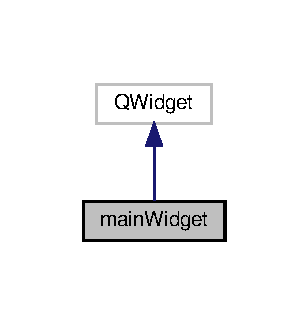
\includegraphics[width=148pt]{classmainWidget__inherit__graph}
\end{center}
\end{figure}


Collaboration diagram for main\+Widget\+:
\nopagebreak
\begin{figure}[H]
\begin{center}
\leavevmode
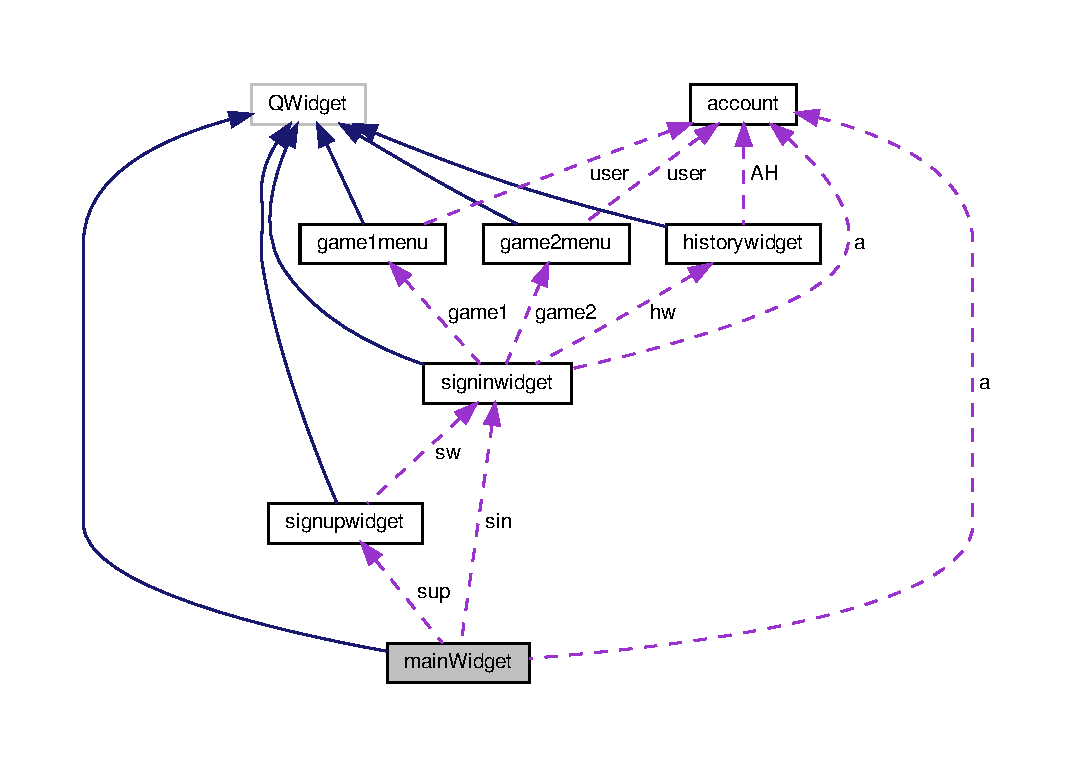
\includegraphics[width=350pt]{classmainWidget__coll__graph}
\end{center}
\end{figure}
\subsection*{Public Slots}
\begin{DoxyCompactItemize}
\item 
void \hyperlink{classmainWidget_a18a889384066a82c65b71cd9d26a4dcb}{signin} ()
\begin{DoxyCompactList}\small\item\em signin slot \end{DoxyCompactList}\item 
void \hyperlink{classmainWidget_a90ca9a99780c436835324252d7b97fb8}{signup} ()
\begin{DoxyCompactList}\small\item\em sign up slot \end{DoxyCompactList}\item 
void \hyperlink{classmainWidget_afc358112a27702edf74ff89cc485a8d1}{play\+As\+Guest} ()
\begin{DoxyCompactList}\small\item\em Play as guest slot. \end{DoxyCompactList}\end{DoxyCompactItemize}
\subsection*{Public Member Functions}
\begin{DoxyCompactItemize}
\item 
\hyperlink{classmainWidget_ad73a469a876f7642f125c2e114fde3b6}{main\+Widget} (Q\+Widget $\ast$parent=nullptr)
\begin{DoxyCompactList}\small\item\em main widget constructor \end{DoxyCompactList}\end{DoxyCompactItemize}
\subsection*{Public Attributes}
\begin{DoxyCompactItemize}
\item 
\mbox{\Hypertarget{classmainWidget_a5ef4f48ef805f95c53d0ec0313c7bc89}\label{classmainWidget_a5ef4f48ef805f95c53d0ec0313c7bc89}} 
Q\+Label $\ast$ \hyperlink{classmainWidget_a5ef4f48ef805f95c53d0ec0313c7bc89}{label0}
\begin{DoxyCompactList}\small\item\em user name label \end{DoxyCompactList}\item 
\mbox{\Hypertarget{classmainWidget_a7f7e7275c34bffebe84268c5183de13a}\label{classmainWidget_a7f7e7275c34bffebe84268c5183de13a}} 
Q\+Label $\ast$ \hyperlink{classmainWidget_a7f7e7275c34bffebe84268c5183de13a}{label1}
\begin{DoxyCompactList}\small\item\em password label \end{DoxyCompactList}\item 
\mbox{\Hypertarget{classmainWidget_a18ac25b117347823b13bd426b8d06f83}\label{classmainWidget_a18ac25b117347823b13bd426b8d06f83}} 
Q\+Line\+Edit $\ast$ \hyperlink{classmainWidget_a18ac25b117347823b13bd426b8d06f83}{line0}
\begin{DoxyCompactList}\small\item\em user name line \end{DoxyCompactList}\item 
\mbox{\Hypertarget{classmainWidget_a02d57a5f34d67dbd22a40cccf3f06dea}\label{classmainWidget_a02d57a5f34d67dbd22a40cccf3f06dea}} 
Q\+Line\+Edit $\ast$ \hyperlink{classmainWidget_a02d57a5f34d67dbd22a40cccf3f06dea}{line1}
\begin{DoxyCompactList}\small\item\em password line \end{DoxyCompactList}\item 
\mbox{\Hypertarget{classmainWidget_ae06b06238db14e9778cfc833a19de508}\label{classmainWidget_ae06b06238db14e9778cfc833a19de508}} 
Q\+Push\+Button $\ast$ \hyperlink{classmainWidget_ae06b06238db14e9778cfc833a19de508}{P\+B0}
\begin{DoxyCompactList}\small\item\em sign in button \end{DoxyCompactList}\item 
\mbox{\Hypertarget{classmainWidget_ad3d6eeca72bc2c2b645215788ad99845}\label{classmainWidget_ad3d6eeca72bc2c2b645215788ad99845}} 
Q\+Push\+Button $\ast$ \hyperlink{classmainWidget_ad3d6eeca72bc2c2b645215788ad99845}{P\+B1}
\begin{DoxyCompactList}\small\item\em sign up button \end{DoxyCompactList}\item 
\mbox{\Hypertarget{classmainWidget_aa6695b4c594e1e6bc912e616adc08219}\label{classmainWidget_aa6695b4c594e1e6bc912e616adc08219}} 
Q\+Push\+Button $\ast$ \hyperlink{classmainWidget_aa6695b4c594e1e6bc912e616adc08219}{P\+B2}
\begin{DoxyCompactList}\small\item\em play as guest button \end{DoxyCompactList}\item 
\mbox{\Hypertarget{classmainWidget_a685a23d47d4956f700e126a2e69e3917}\label{classmainWidget_a685a23d47d4956f700e126a2e69e3917}} 
Q\+V\+Box\+Layout $\ast$ \hyperlink{classmainWidget_a685a23d47d4956f700e126a2e69e3917}{V\+Box}
\begin{DoxyCompactList}\small\item\em vertical box layout \end{DoxyCompactList}\item 
\mbox{\Hypertarget{classmainWidget_a96bac6fd934c13f6ded4c43082fc5929}\label{classmainWidget_a96bac6fd934c13f6ded4c43082fc5929}} 
\hyperlink{classsignupwidget}{signupwidget} $\ast$ \hyperlink{classmainWidget_a96bac6fd934c13f6ded4c43082fc5929}{sup}
\begin{DoxyCompactList}\small\item\em sign up widget \end{DoxyCompactList}\item 
\mbox{\Hypertarget{classmainWidget_aa9b41cfbf49f6d720494a0c9576b1fb6}\label{classmainWidget_aa9b41cfbf49f6d720494a0c9576b1fb6}} 
\hyperlink{classaccount}{account} $\ast$ \hyperlink{classmainWidget_aa9b41cfbf49f6d720494a0c9576b1fb6}{a}
\begin{DoxyCompactList}\small\item\em account \end{DoxyCompactList}\item 
\mbox{\Hypertarget{classmainWidget_a0b71164fff8e07af805378dc25820339}\label{classmainWidget_a0b71164fff8e07af805378dc25820339}} 
\hyperlink{classsigninwidget}{signinwidget} $\ast$ \hyperlink{classmainWidget_a0b71164fff8e07af805378dc25820339}{sin}
\begin{DoxyCompactList}\small\item\em sign in widget \end{DoxyCompactList}\item 
\mbox{\Hypertarget{classmainWidget_a0a251b7bb0921be1c12fd446512ab334}\label{classmainWidget_a0a251b7bb0921be1c12fd446512ab334}} 
Q\+Message\+Box $\ast$ \hyperlink{classmainWidget_a0a251b7bb0921be1c12fd446512ab334}{message\+Box}
\begin{DoxyCompactList}\small\item\em messagebox to display errors \end{DoxyCompactList}\end{DoxyCompactItemize}


\subsection{Detailed Description}
contains main widget class defintion 

This class is responsible for constructing the main widget 

\subsection{Constructor \& Destructor Documentation}
\mbox{\Hypertarget{classmainWidget_ad73a469a876f7642f125c2e114fde3b6}\label{classmainWidget_ad73a469a876f7642f125c2e114fde3b6}} 
\index{main\+Widget@{main\+Widget}!main\+Widget@{main\+Widget}}
\index{main\+Widget@{main\+Widget}!main\+Widget@{main\+Widget}}
\subsubsection{\texorpdfstring{main\+Widget()}{mainWidget()}}
{\footnotesize\ttfamily main\+Widget\+::main\+Widget (\begin{DoxyParamCaption}\item[{Q\+Widget $\ast$}]{parent = {\ttfamily nullptr} }\end{DoxyParamCaption})\hspace{0.3cm}{\ttfamily [explicit]}}



main widget constructor 

responsible for building the gui of main widget and linking the buttons to their respective slots 

\subsection{Member Function Documentation}
\mbox{\Hypertarget{classmainWidget_afc358112a27702edf74ff89cc485a8d1}\label{classmainWidget_afc358112a27702edf74ff89cc485a8d1}} 
\index{main\+Widget@{main\+Widget}!play\+As\+Guest@{play\+As\+Guest}}
\index{play\+As\+Guest@{play\+As\+Guest}!main\+Widget@{main\+Widget}}
\subsubsection{\texorpdfstring{play\+As\+Guest}{playAsGuest}}
{\footnotesize\ttfamily void main\+Widget\+::play\+As\+Guest (\begin{DoxyParamCaption}{ }\end{DoxyParamCaption})\hspace{0.3cm}{\ttfamily [slot]}}



Play as guest slot. 

opens sign in widget as a guest and closes main widget and adds guest to the list of users if it is not there. \mbox{\Hypertarget{classmainWidget_a18a889384066a82c65b71cd9d26a4dcb}\label{classmainWidget_a18a889384066a82c65b71cd9d26a4dcb}} 
\index{main\+Widget@{main\+Widget}!signin@{signin}}
\index{signin@{signin}!main\+Widget@{main\+Widget}}
\subsubsection{\texorpdfstring{signin}{signin}}
{\footnotesize\ttfamily void main\+Widget\+::signin (\begin{DoxyParamCaption}{ }\end{DoxyParamCaption})\hspace{0.3cm}{\ttfamily [slot]}}



signin slot 

responsible for checking if the user is in the database and if he typed the password correctly if so opens sign in widget \mbox{\Hypertarget{classmainWidget_a90ca9a99780c436835324252d7b97fb8}\label{classmainWidget_a90ca9a99780c436835324252d7b97fb8}} 
\index{main\+Widget@{main\+Widget}!signup@{signup}}
\index{signup@{signup}!main\+Widget@{main\+Widget}}
\subsubsection{\texorpdfstring{signup}{signup}}
{\footnotesize\ttfamily void main\+Widget\+::signup (\begin{DoxyParamCaption}{ }\end{DoxyParamCaption})\hspace{0.3cm}{\ttfamily [slot]}}



sign up slot 

open sign up widget and closes main widget 

The documentation for this class was generated from the following files\+:\begin{DoxyCompactItemize}
\item 
\hyperlink{mainwidget_8h}{mainwidget.\+h}\item 
mainwidget.\+cpp\end{DoxyCompactItemize}

\hypertarget{classpiece}{}\section{piece Class Reference}
\label{classpiece}\index{piece@{piece}}


contains piece class definition  




{\ttfamily \#include $<$piece.\+h$>$}



Inheritance diagram for piece\+:\nopagebreak
\begin{figure}[H]
\begin{center}
\leavevmode
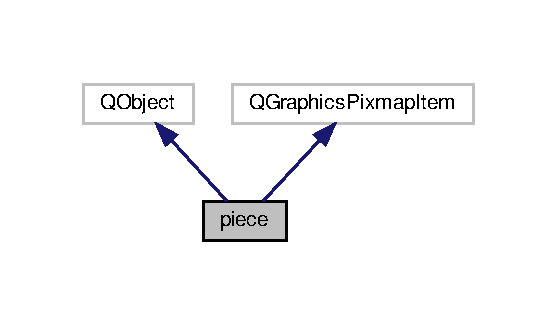
\includegraphics[width=268pt]{classpiece__inherit__graph}
\end{center}
\end{figure}


Collaboration diagram for piece\+:\nopagebreak
\begin{figure}[H]
\begin{center}
\leavevmode
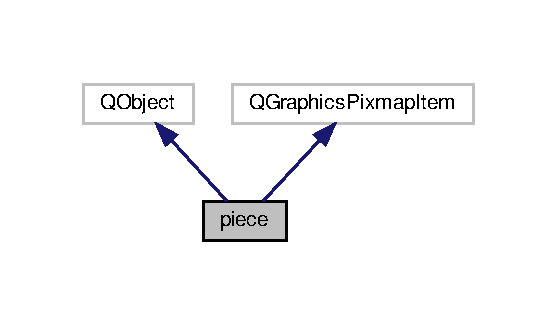
\includegraphics[width=268pt]{classpiece__coll__graph}
\end{center}
\end{figure}
\subsection*{Public Types}
\begin{DoxyCompactItemize}
\item 
\mbox{\Hypertarget{classpiece_a73c0d56d279ed4910cfc0e95ca40be6e}\label{classpiece_a73c0d56d279ed4910cfc0e95ca40be6e}} 
enum {\bfseries state} \{ {\bfseries invalid}, 
{\bfseries valid}, 
{\bfseries white}, 
{\bfseries black}
 \}
\end{DoxyCompactItemize}
\subsection*{Public Slots}
\begin{DoxyCompactItemize}
\item 
void \hyperlink{classpiece_a8db42fa9c9e1b03f3a68f238546ab239}{place} ()
\begin{DoxyCompactList}\small\item\em places a piece. \end{DoxyCompactList}\end{DoxyCompactItemize}
\subsection*{Signals}
\begin{DoxyCompactItemize}
\item 
void \hyperlink{classpiece_a57ea505efe23d31353611198296a5a5a}{placed} ()
\begin{DoxyCompactList}\small\item\em signal to be emitted. \end{DoxyCompactList}\end{DoxyCompactItemize}
\subsection*{Public Member Functions}
\begin{DoxyCompactItemize}
\item 
\hyperlink{classpiece_a65fb95a430bc20242a04556dc1d8bd65}{piece} (Q\+Object $\ast$parent=nullptr)
\begin{DoxyCompactList}\small\item\em piece constructor. \end{DoxyCompactList}\item 
void \hyperlink{classpiece_a899f04d950ea038a6784cba40a1e4289}{set\+State} (state \hyperlink{classpiece_abefadbf9b67a599b3aef7c6fcb731365}{s})
\begin{DoxyCompactList}\small\item\em sets the state of a piece. \end{DoxyCompactList}\end{DoxyCompactItemize}
\subsection*{Public Attributes}
\begin{DoxyCompactItemize}
\item 
\mbox{\Hypertarget{classpiece_abefadbf9b67a599b3aef7c6fcb731365}\label{classpiece_abefadbf9b67a599b3aef7c6fcb731365}} 
state \hyperlink{classpiece_abefadbf9b67a599b3aef7c6fcb731365}{s}
\begin{DoxyCompactList}\small\item\em indicates the state of a piece \end{DoxyCompactList}\item 
\mbox{\Hypertarget{classpiece_a6bb48a39b35cc414ac7f8e3dc175558f}\label{classpiece_a6bb48a39b35cc414ac7f8e3dc175558f}} 
bool \hyperlink{classpiece_a6bb48a39b35cc414ac7f8e3dc175558f}{fresh}
\begin{DoxyCompactList}\small\item\em bool value to store if the piece is the newest piece on the board \end{DoxyCompactList}\item 
\mbox{\Hypertarget{classpiece_a070e7829edca743adda436de84161999}\label{classpiece_a070e7829edca743adda436de84161999}} 
Q\+Media\+Player $\ast$ \hyperlink{classpiece_a070e7829edca743adda436de84161999}{placep}
\begin{DoxyCompactList}\small\item\em audio to be played when a piece is placed \end{DoxyCompactList}\end{DoxyCompactItemize}


\subsection{Detailed Description}
contains piece class definition 

This class is responsible for placing a piece in game 2 and displaying it on the screen 

\subsection{Constructor \& Destructor Documentation}
\mbox{\Hypertarget{classpiece_a65fb95a430bc20242a04556dc1d8bd65}\label{classpiece_a65fb95a430bc20242a04556dc1d8bd65}} 
\index{piece@{piece}!piece@{piece}}
\index{piece@{piece}!piece@{piece}}
\subsubsection{\texorpdfstring{piece()}{piece()}}
{\footnotesize\ttfamily piece\+::piece (\begin{DoxyParamCaption}\item[{Q\+Object $\ast$}]{parent = {\ttfamily nullptr} }\end{DoxyParamCaption})\hspace{0.3cm}{\ttfamily [explicit]}}



piece constructor. 

constructor was only used to set the media player and timers. 

\subsection{Member Function Documentation}
\mbox{\Hypertarget{classpiece_a8db42fa9c9e1b03f3a68f238546ab239}\label{classpiece_a8db42fa9c9e1b03f3a68f238546ab239}} 
\index{piece@{piece}!place@{place}}
\index{place@{place}!piece@{piece}}
\subsubsection{\texorpdfstring{place}{place}}
{\footnotesize\ttfamily void piece\+::place (\begin{DoxyParamCaption}{ }\end{DoxyParamCaption})\hspace{0.3cm}{\ttfamily [slot]}}



places a piece. 

when a valid piece is selected it\textquotesingle{}s state is replaced by eithe white or black depending on the turn. In addition to that, the place audio is played and a signal is emitted to \hyperlink{classgame2scene}{game2scene}. \mbox{\Hypertarget{classpiece_a57ea505efe23d31353611198296a5a5a}\label{classpiece_a57ea505efe23d31353611198296a5a5a}} 
\index{piece@{piece}!placed@{placed}}
\index{placed@{placed}!piece@{piece}}
\subsubsection{\texorpdfstring{placed}{placed}}
{\footnotesize\ttfamily void piece\+::placed (\begin{DoxyParamCaption}{ }\end{DoxyParamCaption})\hspace{0.3cm}{\ttfamily [signal]}}



signal to be emitted. 

signal to be emitted to \hyperlink{classgame2scene}{game2scene} to indicate that a piece is placed. \mbox{\Hypertarget{classpiece_a899f04d950ea038a6784cba40a1e4289}\label{classpiece_a899f04d950ea038a6784cba40a1e4289}} 
\index{piece@{piece}!set\+State@{set\+State}}
\index{set\+State@{set\+State}!piece@{piece}}
\subsubsection{\texorpdfstring{set\+State()}{setState()}}
{\footnotesize\ttfamily void piece\+::set\+State (\begin{DoxyParamCaption}\item[{state}]{s }\end{DoxyParamCaption})}



sets the state of a piece. 

sets the state of a piece and displays the correct image (black circle, white circle, green box, yellow box). 

The documentation for this class was generated from the following files\+:\begin{DoxyCompactItemize}
\item 
piece.\+h\item 
piece.\+cpp\end{DoxyCompactItemize}

\hypertarget{classsigninwidget}{}\section{signinwidget Class Reference}
\label{classsigninwidget}\index{signinwidget@{signinwidget}}


contains signin widget class defintion  




{\ttfamily \#include $<$signinwidget.\+h$>$}



Inheritance diagram for signinwidget\+:\nopagebreak
\begin{figure}[H]
\begin{center}
\leavevmode
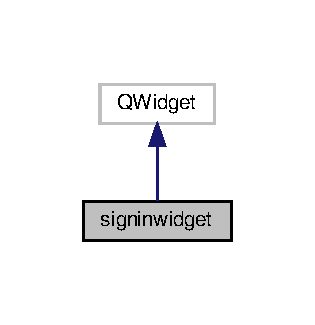
\includegraphics[width=151pt]{classsigninwidget__inherit__graph}
\end{center}
\end{figure}


Collaboration diagram for signinwidget\+:
\nopagebreak
\begin{figure}[H]
\begin{center}
\leavevmode
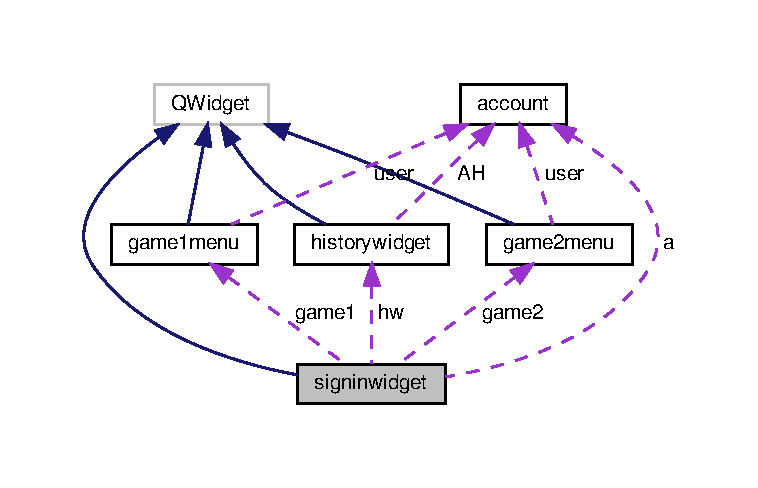
\includegraphics[width=350pt]{classsigninwidget__coll__graph}
\end{center}
\end{figure}
\subsection*{Public Slots}
\begin{DoxyCompactItemize}
\item 
void \hyperlink{classsigninwidget_ad65d01b8dfc345ec25de223a989fd074}{History} ()
\begin{DoxyCompactList}\small\item\em History button slot. \end{DoxyCompactList}\item 
void \hyperlink{classsigninwidget_a885c28fa8a2f7bb105049645f6b28de9}{play\+Game1} ()
\begin{DoxyCompactList}\small\item\em Play game1 button. \end{DoxyCompactList}\item 
void \hyperlink{classsigninwidget_a5f450a4cfdb5151fd1e3254f094d0265}{play\+Game2} ()
\begin{DoxyCompactList}\small\item\em Play game 2 button. \end{DoxyCompactList}\item 
void \hyperlink{classsigninwidget_a873db27ec0eb7d4b758fac6d8f39519a}{quit} ()
\begin{DoxyCompactList}\small\item\em quit button \end{DoxyCompactList}\end{DoxyCompactItemize}
\subsection*{Public Member Functions}
\begin{DoxyCompactItemize}
\item 
\hyperlink{classsigninwidget_aee9526f175ba0bdd88438b7b0d26b99d}{signinwidget} (Q\+Widget $\ast$parent=nullptr)
\begin{DoxyCompactList}\small\item\em signin widget constructor \end{DoxyCompactList}\item 
void \hyperlink{classsigninwidget_a718e8f00822a5386e064765def03d4a7}{get\+Name} ()
\begin{DoxyCompactList}\small\item\em get name function \end{DoxyCompactList}\item 
void \hyperlink{classsigninwidget_a224d1d91ae499107379f886fbd9bec88}{check\+Birthday} ()
\begin{DoxyCompactList}\small\item\em Checking birthday function. \end{DoxyCompactList}\end{DoxyCompactItemize}
\subsection*{Public Attributes}
\begin{DoxyCompactItemize}
\item 
\mbox{\Hypertarget{classsigninwidget_a57cc4742680c09df298a2c3440a5620a}\label{classsigninwidget_a57cc4742680c09df298a2c3440a5620a}} 
\hyperlink{classaccount}{account} $\ast$ \hyperlink{classsigninwidget_a57cc4742680c09df298a2c3440a5620a}{a}
\begin{DoxyCompactList}\small\item\em account of user who signed in \end{DoxyCompactList}\item 
\mbox{\Hypertarget{classsigninwidget_afc822cc2d8fe3d8be04c697257858fd7}\label{classsigninwidget_afc822cc2d8fe3d8be04c697257858fd7}} 
\hyperlink{classgame1menu}{game1menu} $\ast$ \hyperlink{classsigninwidget_afc822cc2d8fe3d8be04c697257858fd7}{game1}
\begin{DoxyCompactList}\small\item\em game1 menu \end{DoxyCompactList}\item 
\mbox{\Hypertarget{classsigninwidget_a3f15f1da5a52cb4ff98c1ce28f8a8dbb}\label{classsigninwidget_a3f15f1da5a52cb4ff98c1ce28f8a8dbb}} 
\hyperlink{classgame2menu}{game2menu} $\ast$ \hyperlink{classsigninwidget_a3f15f1da5a52cb4ff98c1ce28f8a8dbb}{game2}
\begin{DoxyCompactList}\small\item\em game2 menu \end{DoxyCompactList}\item 
\mbox{\Hypertarget{classsigninwidget_ac6259613d09c160b64273541ae19935a}\label{classsigninwidget_ac6259613d09c160b64273541ae19935a}} 
\hyperlink{classhistorywidget}{historywidget} $\ast$ \hyperlink{classsigninwidget_ac6259613d09c160b64273541ae19935a}{hw}
\begin{DoxyCompactList}\small\item\em the history widget \end{DoxyCompactList}\item 
\mbox{\Hypertarget{classsigninwidget_a0ae5b573072a02890e831d5087377fb7}\label{classsigninwidget_a0ae5b573072a02890e831d5087377fb7}} 
Q\+Label $\ast$ \hyperlink{classsigninwidget_a0ae5b573072a02890e831d5087377fb7}{pic}
\begin{DoxyCompactList}\small\item\em picture label for profile picture \end{DoxyCompactList}\item 
\mbox{\Hypertarget{classsigninwidget_ac1aca24cebcf22cd77c681a3b0c7f171}\label{classsigninwidget_ac1aca24cebcf22cd77c681a3b0c7f171}} 
Q\+Label $\ast$ \hyperlink{classsigninwidget_ac1aca24cebcf22cd77c681a3b0c7f171}{name}
\begin{DoxyCompactList}\small\item\em name label for the user\textquotesingle{}s name \end{DoxyCompactList}\item 
\mbox{\Hypertarget{classsigninwidget_a812fea770f80db3166d5dc147cf3f69c}\label{classsigninwidget_a812fea770f80db3166d5dc147cf3f69c}} 
Q\+Message\+Box $\ast$ \hyperlink{classsigninwidget_a812fea770f80db3166d5dc147cf3f69c}{message\+Box}
\begin{DoxyCompactList}\small\item\em message box to display birthday congratulations \end{DoxyCompactList}\item 
\mbox{\Hypertarget{classsigninwidget_a63e301fc2747e03bb83530c416a9ed02}\label{classsigninwidget_a63e301fc2747e03bb83530c416a9ed02}} 
Q\+Push\+Button $\ast$ \hyperlink{classsigninwidget_a63e301fc2747e03bb83530c416a9ed02}{history}
\begin{DoxyCompactList}\small\item\em history button \end{DoxyCompactList}\item 
\mbox{\Hypertarget{classsigninwidget_a088b44ef57dbd41f053ee997f4f4459f}\label{classsigninwidget_a088b44ef57dbd41f053ee997f4f4459f}} 
Q\+Push\+Button $\ast$ \hyperlink{classsigninwidget_a088b44ef57dbd41f053ee997f4f4459f}{play1}
\begin{DoxyCompactList}\small\item\em game 1 button \end{DoxyCompactList}\item 
\mbox{\Hypertarget{classsigninwidget_a30ca5a2ce91444bee74773b146df45a3}\label{classsigninwidget_a30ca5a2ce91444bee74773b146df45a3}} 
Q\+Push\+Button $\ast$ \hyperlink{classsigninwidget_a30ca5a2ce91444bee74773b146df45a3}{play2}
\begin{DoxyCompactList}\small\item\em game 2 button \end{DoxyCompactList}\item 
\mbox{\Hypertarget{classsigninwidget_a37c87918de3d570ad763b5b95282dd48}\label{classsigninwidget_a37c87918de3d570ad763b5b95282dd48}} 
Q\+Push\+Button $\ast$ \hyperlink{classsigninwidget_a37c87918de3d570ad763b5b95282dd48}{logout}
\begin{DoxyCompactList}\small\item\em logout button \end{DoxyCompactList}\item 
\mbox{\Hypertarget{classsigninwidget_a48eb142e986e092a97a2cb8e1097c73d}\label{classsigninwidget_a48eb142e986e092a97a2cb8e1097c73d}} 
Q\+V\+Box\+Layout $\ast$ \hyperlink{classsigninwidget_a48eb142e986e092a97a2cb8e1097c73d}{V\+Box}
\begin{DoxyCompactList}\small\item\em vertical box layout \end{DoxyCompactList}\item 
\mbox{\Hypertarget{classsigninwidget_a31bf8a7eafb4e519397466aec3a26f60}\label{classsigninwidget_a31bf8a7eafb4e519397466aec3a26f60}} 
Q\+Image $\ast$ \hyperlink{classsigninwidget_a31bf8a7eafb4e519397466aec3a26f60}{image}
\begin{DoxyCompactList}\small\item\em image for profile pic \end{DoxyCompactList}\end{DoxyCompactItemize}


\subsection{Detailed Description}
contains signin widget class defintion 

This class is responsible for constructing the signin widget 

\subsection{Constructor \& Destructor Documentation}
\mbox{\Hypertarget{classsigninwidget_aee9526f175ba0bdd88438b7b0d26b99d}\label{classsigninwidget_aee9526f175ba0bdd88438b7b0d26b99d}} 
\index{signinwidget@{signinwidget}!signinwidget@{signinwidget}}
\index{signinwidget@{signinwidget}!signinwidget@{signinwidget}}
\subsubsection{\texorpdfstring{signinwidget()}{signinwidget()}}
{\footnotesize\ttfamily signinwidget\+::signinwidget (\begin{DoxyParamCaption}\item[{Q\+Widget $\ast$}]{parent = {\ttfamily nullptr} }\end{DoxyParamCaption})\hspace{0.3cm}{\ttfamily [explicit]}}



signin widget constructor 

responsible for building the gui of signin widget and linking the buttons to their respective slots 

\subsection{Member Function Documentation}
\mbox{\Hypertarget{classsigninwidget_a224d1d91ae499107379f886fbd9bec88}\label{classsigninwidget_a224d1d91ae499107379f886fbd9bec88}} 
\index{signinwidget@{signinwidget}!check\+Birthday@{check\+Birthday}}
\index{check\+Birthday@{check\+Birthday}!signinwidget@{signinwidget}}
\subsubsection{\texorpdfstring{check\+Birthday()}{checkBirthday()}}
{\footnotesize\ttfamily void signinwidget\+::check\+Birthday (\begin{DoxyParamCaption}{ }\end{DoxyParamCaption})}



Checking birthday function. 

responsible to check if it is the user\textquotesingle{}s birthday and if so display congratulations message box \mbox{\Hypertarget{classsigninwidget_a718e8f00822a5386e064765def03d4a7}\label{classsigninwidget_a718e8f00822a5386e064765def03d4a7}} 
\index{signinwidget@{signinwidget}!get\+Name@{get\+Name}}
\index{get\+Name@{get\+Name}!signinwidget@{signinwidget}}
\subsubsection{\texorpdfstring{get\+Name()}{getName()}}
{\footnotesize\ttfamily void signinwidget\+::get\+Name (\begin{DoxyParamCaption}{ }\end{DoxyParamCaption})}



get name function 

responsible for getting accounts information and displaying what is relevant on the widget \mbox{\Hypertarget{classsigninwidget_ad65d01b8dfc345ec25de223a989fd074}\label{classsigninwidget_ad65d01b8dfc345ec25de223a989fd074}} 
\index{signinwidget@{signinwidget}!History@{History}}
\index{History@{History}!signinwidget@{signinwidget}}
\subsubsection{\texorpdfstring{History}{History}}
{\footnotesize\ttfamily void signinwidget\+::\+History (\begin{DoxyParamCaption}{ }\end{DoxyParamCaption})\hspace{0.3cm}{\ttfamily [slot]}}



History button slot. 

responsible for checking the users history and displaying the history widget \mbox{\Hypertarget{classsigninwidget_a885c28fa8a2f7bb105049645f6b28de9}\label{classsigninwidget_a885c28fa8a2f7bb105049645f6b28de9}} 
\index{signinwidget@{signinwidget}!play\+Game1@{play\+Game1}}
\index{play\+Game1@{play\+Game1}!signinwidget@{signinwidget}}
\subsubsection{\texorpdfstring{play\+Game1}{playGame1}}
{\footnotesize\ttfamily void signinwidget\+::play\+Game1 (\begin{DoxyParamCaption}{ }\end{DoxyParamCaption})\hspace{0.3cm}{\ttfamily [slot]}}



Play game1 button. 

opens game 1 menu for the user to play game 1 \mbox{\Hypertarget{classsigninwidget_a5f450a4cfdb5151fd1e3254f094d0265}\label{classsigninwidget_a5f450a4cfdb5151fd1e3254f094d0265}} 
\index{signinwidget@{signinwidget}!play\+Game2@{play\+Game2}}
\index{play\+Game2@{play\+Game2}!signinwidget@{signinwidget}}
\subsubsection{\texorpdfstring{play\+Game2}{playGame2}}
{\footnotesize\ttfamily void signinwidget\+::play\+Game2 (\begin{DoxyParamCaption}{ }\end{DoxyParamCaption})\hspace{0.3cm}{\ttfamily [slot]}}



Play game 2 button. 

opens game 2 menu for the user to play game 2 \mbox{\Hypertarget{classsigninwidget_a873db27ec0eb7d4b758fac6d8f39519a}\label{classsigninwidget_a873db27ec0eb7d4b758fac6d8f39519a}} 
\index{signinwidget@{signinwidget}!quit@{quit}}
\index{quit@{quit}!signinwidget@{signinwidget}}
\subsubsection{\texorpdfstring{quit}{quit}}
{\footnotesize\ttfamily void signinwidget\+::quit (\begin{DoxyParamCaption}{ }\end{DoxyParamCaption})\hspace{0.3cm}{\ttfamily [slot]}}



quit button 

goes back to main widget and closes sign in widget 

The documentation for this class was generated from the following files\+:\begin{DoxyCompactItemize}
\item 
\hyperlink{signinwidget_8h}{signinwidget.\+h}\item 
signinwidget.\+cpp\end{DoxyCompactItemize}

\hypertarget{classsignupwidget}{}\section{signupwidget Class Reference}
\label{classsignupwidget}\index{signupwidget@{signupwidget}}


contains signup widget class defintion  




{\ttfamily \#include $<$signupwidget.\+h$>$}



Inheritance diagram for signupwidget\+:\nopagebreak
\begin{figure}[H]
\begin{center}
\leavevmode
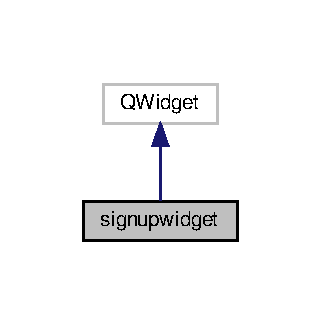
\includegraphics[width=154pt]{classsignupwidget__inherit__graph}
\end{center}
\end{figure}


Collaboration diagram for signupwidget\+:
\nopagebreak
\begin{figure}[H]
\begin{center}
\leavevmode
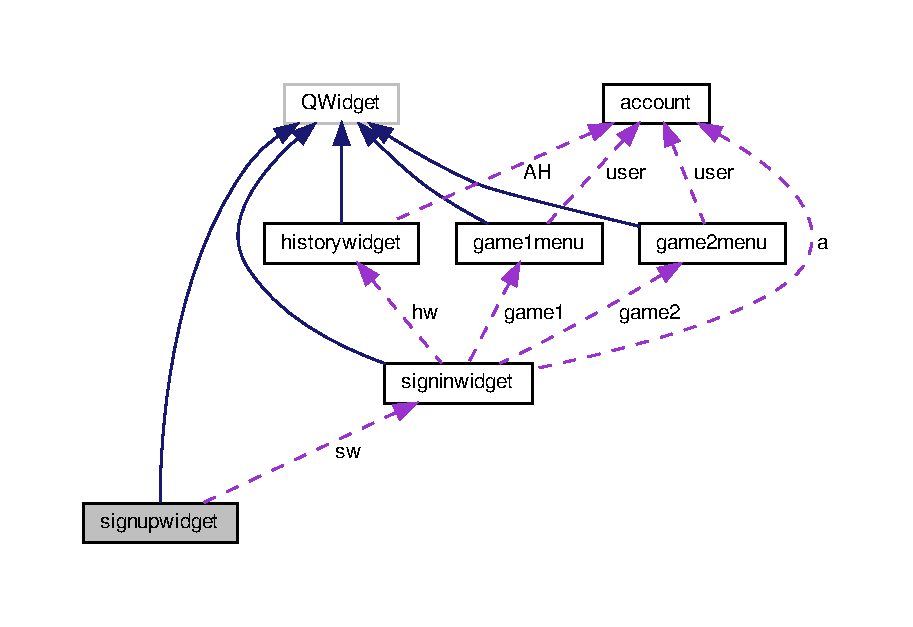
\includegraphics[width=350pt]{classsignupwidget__coll__graph}
\end{center}
\end{figure}
\subsection*{Public Slots}
\begin{DoxyCompactItemize}
\item 
void \hyperlink{classsignupwidget_af3e836d1d5c48db21b8ae0bcaf1e8216}{signup} ()
\begin{DoxyCompactList}\small\item\em sign up button slot \end{DoxyCompactList}\item 
void \hyperlink{classsignupwidget_a70de3f9e8d27a1704a3678d3148f6e46}{image} ()
\begin{DoxyCompactList}\small\item\em image function \end{DoxyCompactList}\item 
void \hyperlink{classsignupwidget_a61682f0dccbdcaa63a4b07434dc52e62}{quit} ()
\begin{DoxyCompactList}\small\item\em quit signup \end{DoxyCompactList}\end{DoxyCompactItemize}
\subsection*{Public Member Functions}
\begin{DoxyCompactItemize}
\item 
\hyperlink{classsignupwidget_a1feed302f7dfc610bba7f28efb1ae554}{signupwidget} (Q\+Widget $\ast$parent=nullptr)
\begin{DoxyCompactList}\small\item\em class constructor \end{DoxyCompactList}\end{DoxyCompactItemize}
\subsection*{Public Attributes}
\begin{DoxyCompactItemize}
\item 
\mbox{\Hypertarget{classsignupwidget_a70b0a263832731e4ad62f234cd81915d}\label{classsignupwidget_a70b0a263832731e4ad62f234cd81915d}} 
Q\+Label $\ast$ \hyperlink{classsignupwidget_a70b0a263832731e4ad62f234cd81915d}{firstname\+\_\+label}
\begin{DoxyCompactList}\small\item\em first name \end{DoxyCompactList}\item 
\mbox{\Hypertarget{classsignupwidget_aade83bff48e4a9b31bd62482d859901d}\label{classsignupwidget_aade83bff48e4a9b31bd62482d859901d}} 
Q\+Label $\ast$ \hyperlink{classsignupwidget_aade83bff48e4a9b31bd62482d859901d}{lastname\+\_\+label}
\begin{DoxyCompactList}\small\item\em last name \end{DoxyCompactList}\item 
\mbox{\Hypertarget{classsignupwidget_a274b82c9dec7bcd59f68b98353cec293}\label{classsignupwidget_a274b82c9dec7bcd59f68b98353cec293}} 
Q\+Label $\ast$ \hyperlink{classsignupwidget_a274b82c9dec7bcd59f68b98353cec293}{username\+\_\+label}
\begin{DoxyCompactList}\small\item\em username \end{DoxyCompactList}\item 
\mbox{\Hypertarget{classsignupwidget_a7776231c96582c1136e5d640612415e3}\label{classsignupwidget_a7776231c96582c1136e5d640612415e3}} 
Q\+Label $\ast$ \hyperlink{classsignupwidget_a7776231c96582c1136e5d640612415e3}{password\+\_\+label}
\begin{DoxyCompactList}\small\item\em password \end{DoxyCompactList}\item 
\mbox{\Hypertarget{classsignupwidget_a6c9efac1ba4ca981bec439e56d5b968b}\label{classsignupwidget_a6c9efac1ba4ca981bec439e56d5b968b}} 
Q\+Label $\ast$ \hyperlink{classsignupwidget_a6c9efac1ba4ca981bec439e56d5b968b}{confirmpassword\+\_\+label}
\begin{DoxyCompactList}\small\item\em confirm password \end{DoxyCompactList}\item 
\mbox{\Hypertarget{classsignupwidget_a561521b369bea3068f4f508f9741eb44}\label{classsignupwidget_a561521b369bea3068f4f508f9741eb44}} 
Q\+Label $\ast$ \hyperlink{classsignupwidget_a561521b369bea3068f4f508f9741eb44}{picture\+\_\+label}
\begin{DoxyCompactList}\small\item\em picture \end{DoxyCompactList}\item 
\mbox{\Hypertarget{classsignupwidget_ad23f07214fdad4b32cbcd0e3a1907a62}\label{classsignupwidget_ad23f07214fdad4b32cbcd0e3a1907a62}} 
Q\+Label $\ast$ \hyperlink{classsignupwidget_ad23f07214fdad4b32cbcd0e3a1907a62}{gender\+\_\+label}
\begin{DoxyCompactList}\small\item\em gender \end{DoxyCompactList}\item 
\mbox{\Hypertarget{classsignupwidget_a548408c62facfa8376cfda78c5fcf956}\label{classsignupwidget_a548408c62facfa8376cfda78c5fcf956}} 
Q\+Label $\ast$ \hyperlink{classsignupwidget_a548408c62facfa8376cfda78c5fcf956}{Date\+Of\+Birth\+\_\+label}
\begin{DoxyCompactList}\small\item\em date of birth \end{DoxyCompactList}\item 
\mbox{\Hypertarget{classsignupwidget_a1bbc9880e3df78d440b2f4014331e50c}\label{classsignupwidget_a1bbc9880e3df78d440b2f4014331e50c}} 
Q\+Line\+Edit $\ast$ \hyperlink{classsignupwidget_a1bbc9880e3df78d440b2f4014331e50c}{firstname\+\_\+line}
\begin{DoxyCompactList}\small\item\em first name \end{DoxyCompactList}\item 
\mbox{\Hypertarget{classsignupwidget_adc3af0488144f497d473631f81c8cb04}\label{classsignupwidget_adc3af0488144f497d473631f81c8cb04}} 
Q\+Line\+Edit $\ast$ \hyperlink{classsignupwidget_adc3af0488144f497d473631f81c8cb04}{lastname\+\_\+line}
\begin{DoxyCompactList}\small\item\em last name \end{DoxyCompactList}\item 
\mbox{\Hypertarget{classsignupwidget_a004c76d8c4f07234c3d9e02a0d538268}\label{classsignupwidget_a004c76d8c4f07234c3d9e02a0d538268}} 
Q\+Line\+Edit $\ast$ \hyperlink{classsignupwidget_a004c76d8c4f07234c3d9e02a0d538268}{username\+\_\+line}
\begin{DoxyCompactList}\small\item\em username \end{DoxyCompactList}\item 
\mbox{\Hypertarget{classsignupwidget_ac476407a39c626a1f6e6163f515c5f83}\label{classsignupwidget_ac476407a39c626a1f6e6163f515c5f83}} 
Q\+Line\+Edit $\ast$ \hyperlink{classsignupwidget_ac476407a39c626a1f6e6163f515c5f83}{password\+\_\+line}
\begin{DoxyCompactList}\small\item\em password \end{DoxyCompactList}\item 
\mbox{\Hypertarget{classsignupwidget_a8dc08eb7b10d9cb9a36d21371c207969}\label{classsignupwidget_a8dc08eb7b10d9cb9a36d21371c207969}} 
Q\+Line\+Edit $\ast$ \hyperlink{classsignupwidget_a8dc08eb7b10d9cb9a36d21371c207969}{comfirmpassword\+\_\+line}
\begin{DoxyCompactList}\small\item\em confirm password \end{DoxyCompactList}\item 
\mbox{\Hypertarget{classsignupwidget_a2affda11d2bdcfc57ea3625e392575df}\label{classsignupwidget_a2affda11d2bdcfc57ea3625e392575df}} 
Q\+Radio\+Button $\ast$ \hyperlink{classsignupwidget_a2affda11d2bdcfc57ea3625e392575df}{R\+B0}
\begin{DoxyCompactList}\small\item\em male RB \end{DoxyCompactList}\item 
\mbox{\Hypertarget{classsignupwidget_ae651f415d5b24bd8cc245cdaee30804e}\label{classsignupwidget_ae651f415d5b24bd8cc245cdaee30804e}} 
Q\+Radio\+Button $\ast$ \hyperlink{classsignupwidget_ae651f415d5b24bd8cc245cdaee30804e}{R\+B1}
\begin{DoxyCompactList}\small\item\em female RB \end{DoxyCompactList}\item 
\mbox{\Hypertarget{classsignupwidget_a78f50024b35dea50931c3c500d4352a4}\label{classsignupwidget_a78f50024b35dea50931c3c500d4352a4}} 
Q\+Calendar\+Widget $\ast$ \hyperlink{classsignupwidget_a78f50024b35dea50931c3c500d4352a4}{C}
\begin{DoxyCompactList}\small\item\em calender widget \end{DoxyCompactList}\item 
\mbox{\Hypertarget{classsignupwidget_a773d4b70414a9f24a9537655c55264b7}\label{classsignupwidget_a773d4b70414a9f24a9537655c55264b7}} 
Q\+Push\+Button $\ast$ \hyperlink{classsignupwidget_a773d4b70414a9f24a9537655c55264b7}{P\+B0}
\begin{DoxyCompactList}\small\item\em sign up \end{DoxyCompactList}\item 
\mbox{\Hypertarget{classsignupwidget_a9aad8c0b558c925ef5d8f70fe4711057}\label{classsignupwidget_a9aad8c0b558c925ef5d8f70fe4711057}} 
Q\+Push\+Button $\ast$ \hyperlink{classsignupwidget_a9aad8c0b558c925ef5d8f70fe4711057}{P\+B1}
\begin{DoxyCompactList}\small\item\em upload pic button \end{DoxyCompactList}\item 
\mbox{\Hypertarget{classsignupwidget_ad4d8d01be423482b316319ce3ba131a2}\label{classsignupwidget_ad4d8d01be423482b316319ce3ba131a2}} 
Q\+Push\+Button $\ast$ \hyperlink{classsignupwidget_ad4d8d01be423482b316319ce3ba131a2}{back}
\begin{DoxyCompactList}\small\item\em back button \end{DoxyCompactList}\item 
\mbox{\Hypertarget{classsignupwidget_ab24ffd3a3a9238cf9d6bfef5f9f306ce}\label{classsignupwidget_ab24ffd3a3a9238cf9d6bfef5f9f306ce}} 
Q\+V\+Box\+Layout $\ast$ \hyperlink{classsignupwidget_ab24ffd3a3a9238cf9d6bfef5f9f306ce}{V\+Box}
\begin{DoxyCompactList}\small\item\em vertical box layout \end{DoxyCompactList}\item 
\mbox{\Hypertarget{classsignupwidget_ac339d7cea970afe1a49dc318b77b4bb2}\label{classsignupwidget_ac339d7cea970afe1a49dc318b77b4bb2}} 
Q\+H\+Box\+Layout $\ast$ \hyperlink{classsignupwidget_ac339d7cea970afe1a49dc318b77b4bb2}{H\+Box}
\begin{DoxyCompactList}\small\item\em horizontal box layout \end{DoxyCompactList}\item 
\mbox{\Hypertarget{classsignupwidget_a3785fe895505fb4513569373617d5d39}\label{classsignupwidget_a3785fe895505fb4513569373617d5d39}} 
Q\+Group\+Box $\ast$ \hyperlink{classsignupwidget_a3785fe895505fb4513569373617d5d39}{G}
\begin{DoxyCompactList}\small\item\em group box \end{DoxyCompactList}\item 
\mbox{\Hypertarget{classsignupwidget_aefc0e695f0cbf575dfdcc6c49746aeeb}\label{classsignupwidget_aefc0e695f0cbf575dfdcc6c49746aeeb}} 
Q\+Message\+Box $\ast$ \hyperlink{classsignupwidget_aefc0e695f0cbf575dfdcc6c49746aeeb}{message\+Box}
\begin{DoxyCompactList}\small\item\em message box displaying errors \end{DoxyCompactList}\item 
\mbox{\Hypertarget{classsignupwidget_aea236de583b2ecc6f8cd0f32c13efc69}\label{classsignupwidget_aea236de583b2ecc6f8cd0f32c13efc69}} 
Q\+Reg\+Exp $\ast$ \hyperlink{classsignupwidget_aea236de583b2ecc6f8cd0f32c13efc69}{password\+\_\+\+Reg\+Ex}
\begin{DoxyCompactList}\small\item\em regular expression used to define the password limits \end{DoxyCompactList}\item 
\mbox{\Hypertarget{classsignupwidget_ace15c8c1f9727aec056771f21970138f}\label{classsignupwidget_ace15c8c1f9727aec056771f21970138f}} 
Q\+String \hyperlink{classsignupwidget_ace15c8c1f9727aec056771f21970138f}{image\+Name} =\char`\"{}\char`\"{}
\begin{DoxyCompactList}\small\item\em filepath as a string for image of user initialized to null \end{DoxyCompactList}\item 
\mbox{\Hypertarget{classsignupwidget_ad694d3ea2e0c93e23d76b1444690db89}\label{classsignupwidget_ad694d3ea2e0c93e23d76b1444690db89}} 
\hyperlink{classsigninwidget}{signinwidget} $\ast$ \hyperlink{classsignupwidget_ad694d3ea2e0c93e23d76b1444690db89}{sw}
\begin{DoxyCompactList}\small\item\em sign in widget to take the user to sign in directly after sign up \end{DoxyCompactList}\end{DoxyCompactItemize}


\subsection{Detailed Description}
contains signup widget class defintion 

This class is responsible for constructing the sign up widget 

\subsection{Constructor \& Destructor Documentation}
\mbox{\Hypertarget{classsignupwidget_a1feed302f7dfc610bba7f28efb1ae554}\label{classsignupwidget_a1feed302f7dfc610bba7f28efb1ae554}} 
\index{signupwidget@{signupwidget}!signupwidget@{signupwidget}}
\index{signupwidget@{signupwidget}!signupwidget@{signupwidget}}
\subsubsection{\texorpdfstring{signupwidget()}{signupwidget()}}
{\footnotesize\ttfamily signupwidget\+::signupwidget (\begin{DoxyParamCaption}\item[{Q\+Widget $\ast$}]{parent = {\ttfamily nullptr} }\end{DoxyParamCaption})\hspace{0.3cm}{\ttfamily [explicit]}}



class constructor 

responsible for constructing the gui and linking the buttons to their respective slot functions 

\subsection{Member Function Documentation}
\mbox{\Hypertarget{classsignupwidget_a70de3f9e8d27a1704a3678d3148f6e46}\label{classsignupwidget_a70de3f9e8d27a1704a3678d3148f6e46}} 
\index{signupwidget@{signupwidget}!image@{image}}
\index{image@{image}!signupwidget@{signupwidget}}
\subsubsection{\texorpdfstring{image}{image}}
{\footnotesize\ttfamily void signupwidget\+::image (\begin{DoxyParamCaption}{ }\end{DoxyParamCaption})\hspace{0.3cm}{\ttfamily [slot]}}



image function 

saves the image to our build directory to have it on next launch \mbox{\Hypertarget{classsignupwidget_a61682f0dccbdcaa63a4b07434dc52e62}\label{classsignupwidget_a61682f0dccbdcaa63a4b07434dc52e62}} 
\index{signupwidget@{signupwidget}!quit@{quit}}
\index{quit@{quit}!signupwidget@{signupwidget}}
\subsubsection{\texorpdfstring{quit}{quit}}
{\footnotesize\ttfamily void signupwidget\+::quit (\begin{DoxyParamCaption}{ }\end{DoxyParamCaption})\hspace{0.3cm}{\ttfamily [slot]}}



quit signup 

takes the user back from sign up widget to main widget \mbox{\Hypertarget{classsignupwidget_af3e836d1d5c48db21b8ae0bcaf1e8216}\label{classsignupwidget_af3e836d1d5c48db21b8ae0bcaf1e8216}} 
\index{signupwidget@{signupwidget}!signup@{signup}}
\index{signup@{signup}!signupwidget@{signupwidget}}
\subsubsection{\texorpdfstring{signup}{signup}}
{\footnotesize\ttfamily void signupwidget\+::signup (\begin{DoxyParamCaption}{ }\end{DoxyParamCaption})\hspace{0.3cm}{\ttfamily [slot]}}



sign up button slot 

responsible for checking if all information is valid and saving the user in the database and signing them in 

The documentation for this class was generated from the following files\+:\begin{DoxyCompactItemize}
\item 
\hyperlink{signupwidget_8h}{signupwidget.\+h}\item 
signupwidget.\+cpp\end{DoxyCompactItemize}

\hypertarget{classvdeath}{}\section{vdeath Class Reference}
\label{classvdeath}\index{vdeath@{vdeath}}


contains virus death class definition  




{\ttfamily \#include $<$vdeath.\+h$>$}



Inheritance diagram for vdeath\+:\nopagebreak
\begin{figure}[H]
\begin{center}
\leavevmode
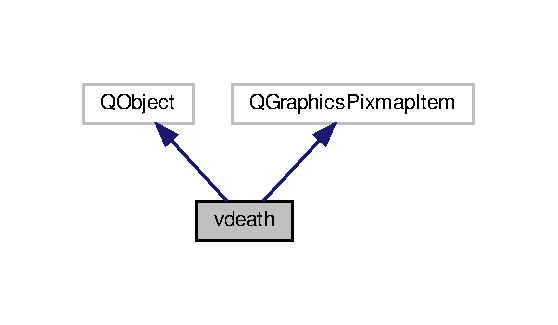
\includegraphics[width=268pt]{classvdeath__inherit__graph}
\end{center}
\end{figure}


Collaboration diagram for vdeath\+:\nopagebreak
\begin{figure}[H]
\begin{center}
\leavevmode
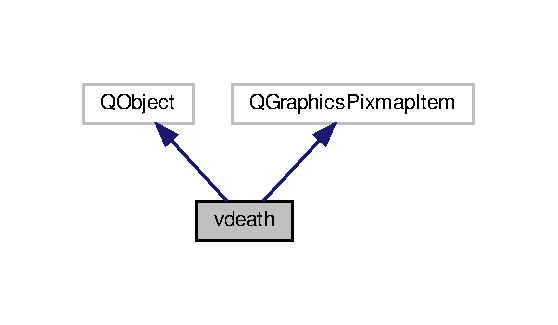
\includegraphics[width=268pt]{classvdeath__coll__graph}
\end{center}
\end{figure}
\subsection*{Public Slots}
\begin{DoxyCompactItemize}
\item 
void \hyperlink{classvdeath_a36a74d88a906688ff06503b61c57b670}{die} ()
\begin{DoxyCompactList}\small\item\em Remove death image from scene. \end{DoxyCompactList}\end{DoxyCompactItemize}
\subsection*{Public Member Functions}
\begin{DoxyCompactItemize}
\item 
\hyperlink{classvdeath_a2b34067182c4e7773baa6cf99d1cf03d}{vdeath} (Q\+Object $\ast$parent=nullptr)
\begin{DoxyCompactList}\small\item\em sets the death image and calls slot die to remove it \end{DoxyCompactList}\end{DoxyCompactItemize}
\subsection*{Public Attributes}
\begin{DoxyCompactItemize}
\item 
\mbox{\Hypertarget{classvdeath_ada84c7cc3712f6801b1a8043df9449e2}\label{classvdeath_ada84c7cc3712f6801b1a8043df9449e2}} 
Q\+Timer $\ast$ \hyperlink{classvdeath_ada84c7cc3712f6801b1a8043df9449e2}{timer}
\begin{DoxyCompactList}\small\item\em timer to remove the death image \end{DoxyCompactList}\end{DoxyCompactItemize}


\subsection{Detailed Description}
contains virus death class definition 

This class is responsible for setting the death animation and removing it from the scene 

\subsection{Constructor \& Destructor Documentation}
\mbox{\Hypertarget{classvdeath_a2b34067182c4e7773baa6cf99d1cf03d}\label{classvdeath_a2b34067182c4e7773baa6cf99d1cf03d}} 
\index{vdeath@{vdeath}!vdeath@{vdeath}}
\index{vdeath@{vdeath}!vdeath@{vdeath}}
\subsubsection{\texorpdfstring{vdeath()}{vdeath()}}
{\footnotesize\ttfamily vdeath\+::vdeath (\begin{DoxyParamCaption}\item[{Q\+Object $\ast$}]{parent = {\ttfamily nullptr} }\end{DoxyParamCaption})\hspace{0.3cm}{\ttfamily [explicit]}}



sets the death image and calls slot die to remove it 

constructor to set the death image and call slot die to remove it from the scene 

\subsection{Member Function Documentation}
\mbox{\Hypertarget{classvdeath_a36a74d88a906688ff06503b61c57b670}\label{classvdeath_a36a74d88a906688ff06503b61c57b670}} 
\index{vdeath@{vdeath}!die@{die}}
\index{die@{die}!vdeath@{vdeath}}
\subsubsection{\texorpdfstring{die}{die}}
{\footnotesize\ttfamily void vdeath\+::die (\begin{DoxyParamCaption}{ }\end{DoxyParamCaption})\hspace{0.3cm}{\ttfamily [slot]}}



Remove death image from scene. 

clearing up the scene from the dead viruses 

The documentation for this class was generated from the following files\+:\begin{DoxyCompactItemize}
\item 
\hyperlink{vdeath_8h}{vdeath.\+h}\item 
vdeath.\+cpp\end{DoxyCompactItemize}

\hypertarget{classvirus}{}\section{virus Class Reference}
\label{classvirus}\index{virus@{virus}}


contains virus class definition  




{\ttfamily \#include $<$virus.\+h$>$}



Inheritance diagram for virus\+:\nopagebreak
\begin{figure}[H]
\begin{center}
\leavevmode
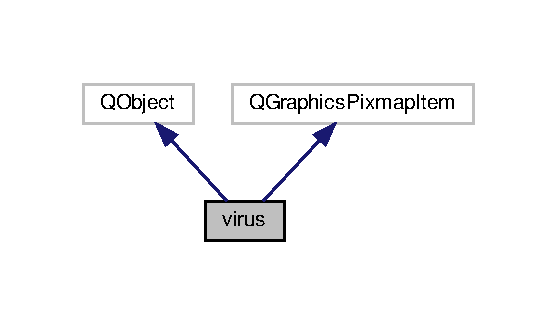
\includegraphics[width=268pt]{classvirus__inherit__graph}
\end{center}
\end{figure}


Collaboration diagram for virus\+:\nopagebreak
\begin{figure}[H]
\begin{center}
\leavevmode
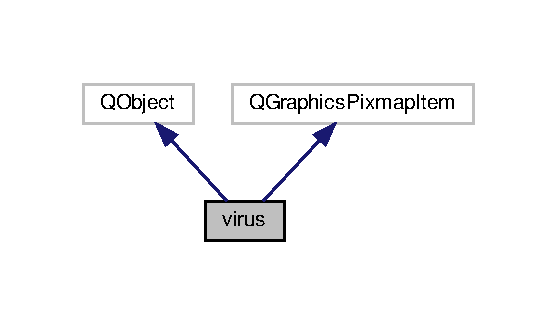
\includegraphics[width=268pt]{classvirus__coll__graph}
\end{center}
\end{figure}
\subsection*{Public Types}
\begin{DoxyCompactItemize}
\item 
\mbox{\Hypertarget{classvirus_a6bd2aa8d6e7d98fab2229f660853fb19}\label{classvirus_a6bd2aa8d6e7d98fab2229f660853fb19}} 
enum {\bfseries sizz} \{ {\bfseries small}, 
{\bfseries medium}, 
{\bfseries big}
 \}
\end{DoxyCompactItemize}
\subsection*{Public Slots}
\begin{DoxyCompactItemize}
\item 
void \hyperlink{classvirus_a8b036fc788433ad3a705e9de6de41ee2}{update} ()
\begin{DoxyCompactList}\small\item\em Updates position of the virus. \end{DoxyCompactList}\item 
void \hyperlink{classvirus_a456b60cbaeed1b370a7f668111e34401}{kill} ()
\begin{DoxyCompactList}\small\item\em Check if virus is selected then kill it. \end{DoxyCompactList}\end{DoxyCompactItemize}
\subsection*{Public Member Functions}
\begin{DoxyCompactItemize}
\item 
\hyperlink{classvirus_aec80936bff04cb885c64075219835d45}{virus} (Q\+Object $\ast$parent=nullptr)
\begin{DoxyCompactList}\small\item\em sets the death sound mediaplayer \end{DoxyCompactList}\item 
void \hyperlink{classvirus_a7e52ed4f11deb1997a7fdbc07c7b038a}{set\+Size} (sizz s)
\begin{DoxyCompactList}\small\item\em sets the size and image to viruses \end{DoxyCompactList}\end{DoxyCompactItemize}
\subsection*{Public Attributes}
\begin{DoxyCompactItemize}
\item 
\mbox{\Hypertarget{classvirus_a469edc5ead8feec20ffa4416b17120de}\label{classvirus_a469edc5ead8feec20ffa4416b17120de}} 
sizz \hyperlink{classvirus_a469edc5ead8feec20ffa4416b17120de}{size}
\begin{DoxyCompactList}\small\item\em instance of enum type \end{DoxyCompactList}\item 
\mbox{\Hypertarget{classvirus_a730412dbb1c4ff0cda46f7ed46c211cd}\label{classvirus_a730412dbb1c4ff0cda46f7ed46c211cd}} 
bool \hyperlink{classvirus_a730412dbb1c4ff0cda46f7ed46c211cd}{alive}
\begin{DoxyCompactList}\small\item\em boolean to verify if virus is alive \end{DoxyCompactList}\item 
\mbox{\Hypertarget{classvirus_a26cc1e0617d779ab9cecea2ccb3833e3}\label{classvirus_a26cc1e0617d779ab9cecea2ccb3833e3}} 
bool \hyperlink{classvirus_a26cc1e0617d779ab9cecea2ccb3833e3}{is\+Checked}
\begin{DoxyCompactList}\small\item\em used to keep track for score \end{DoxyCompactList}\item 
\mbox{\Hypertarget{classvirus_af3db844b2d5e6c48f6810c5783c140ed}\label{classvirus_af3db844b2d5e6c48f6810c5783c140ed}} 
Q\+Media\+Player $\ast$ \hyperlink{classvirus_af3db844b2d5e6c48f6810c5783c140ed}{deathsound}
\begin{DoxyCompactList}\small\item\em mediaplayer to play death sound \end{DoxyCompactList}\item 
\mbox{\Hypertarget{classvirus_af952b682874f8080fea53718dc136874}\label{classvirus_af952b682874f8080fea53718dc136874}} 
int \hyperlink{classvirus_af952b682874f8080fea53718dc136874}{speed}
\begin{DoxyCompactList}\small\item\em speed of viruses falling \end{DoxyCompactList}\item 
\mbox{\Hypertarget{classvirus_ab7a1a248f91d2826090771212b62681f}\label{classvirus_ab7a1a248f91d2826090771212b62681f}} 
Q\+Timer $\ast$ \hyperlink{classvirus_ab7a1a248f91d2826090771212b62681f}{timer}
\begin{DoxyCompactList}\small\item\em first timer responsible for calling update position of virus \end{DoxyCompactList}\item 
\mbox{\Hypertarget{classvirus_a7fee7454da0a4960783f23fbfa42e1c7}\label{classvirus_a7fee7454da0a4960783f23fbfa42e1c7}} 
Q\+Timer $\ast$ \hyperlink{classvirus_a7fee7454da0a4960783f23fbfa42e1c7}{timer2}
\begin{DoxyCompactList}\small\item\em second timer responsible for calling kill to check for killed viruses \end{DoxyCompactList}\end{DoxyCompactItemize}


\subsection{Detailed Description}
contains virus class definition 

This class is responsible for creating the viruses for the game along with destroying them on click 

\subsection{Constructor \& Destructor Documentation}
\mbox{\Hypertarget{classvirus_aec80936bff04cb885c64075219835d45}\label{classvirus_aec80936bff04cb885c64075219835d45}} 
\index{virus@{virus}!virus@{virus}}
\index{virus@{virus}!virus@{virus}}
\subsubsection{\texorpdfstring{virus()}{virus()}}
{\footnotesize\ttfamily virus\+::virus (\begin{DoxyParamCaption}\item[{Q\+Object $\ast$}]{parent = {\ttfamily nullptr} }\end{DoxyParamCaption})\hspace{0.3cm}{\ttfamily [explicit]}}



sets the death sound mediaplayer 

constructor was only used to set the media player other functionalities were delegated to \hyperlink{classvirus_a7e52ed4f11deb1997a7fdbc07c7b038a}{set\+Size()} 

\subsection{Member Function Documentation}
\mbox{\Hypertarget{classvirus_a456b60cbaeed1b370a7f668111e34401}\label{classvirus_a456b60cbaeed1b370a7f668111e34401}} 
\index{virus@{virus}!kill@{kill}}
\index{kill@{kill}!virus@{virus}}
\subsubsection{\texorpdfstring{kill}{kill}}
{\footnotesize\ttfamily void virus\+::kill (\begin{DoxyParamCaption}{ }\end{DoxyParamCaption})\hspace{0.3cm}{\ttfamily [slot]}}



Check if virus is selected then kill it. 

checks if a virus was selected then it kills it and plays the deathsound and displays death animation \mbox{\Hypertarget{classvirus_a7e52ed4f11deb1997a7fdbc07c7b038a}\label{classvirus_a7e52ed4f11deb1997a7fdbc07c7b038a}} 
\index{virus@{virus}!set\+Size@{set\+Size}}
\index{set\+Size@{set\+Size}!virus@{virus}}
\subsubsection{\texorpdfstring{set\+Size()}{setSize()}}
{\footnotesize\ttfamily void virus\+::set\+Size (\begin{DoxyParamCaption}\item[{sizz}]{s }\end{DoxyParamCaption})}



sets the size and image to viruses 

sets the size of the virus along with a respective image and connects the timers to their respective slots. to be called everytime you need to create a virus. \mbox{\Hypertarget{classvirus_a8b036fc788433ad3a705e9de6de41ee2}\label{classvirus_a8b036fc788433ad3a705e9de6de41ee2}} 
\index{virus@{virus}!update@{update}}
\index{update@{update}!virus@{virus}}
\subsubsection{\texorpdfstring{update}{update}}
{\footnotesize\ttfamily void virus\+::update (\begin{DoxyParamCaption}{ }\end{DoxyParamCaption})\hspace{0.3cm}{\ttfamily [slot]}}



Updates position of the virus. 

make the virus fall down with varrying speeds. 

The documentation for this class was generated from the following files\+:\begin{DoxyCompactItemize}
\item 
\hyperlink{virus_8h}{virus.\+h}\item 
virus.\+cpp\end{DoxyCompactItemize}

\chapter{File Documentation}
\input{account_8h}
\hypertarget{button_8h}{}\section{button.\+h File Reference}
\label{button_8h}\index{button.\+h@{button.\+h}}


contains button class definition  


{\ttfamily \#include $<$Q\+Graphics\+Rect\+Item$>$}\newline
{\ttfamily \#include $<$Q\+Graphics\+Scene\+Mouse\+Event$>$}\newline
Include dependency graph for button.\+h\+:\nopagebreak
\begin{figure}[H]
\begin{center}
\leavevmode
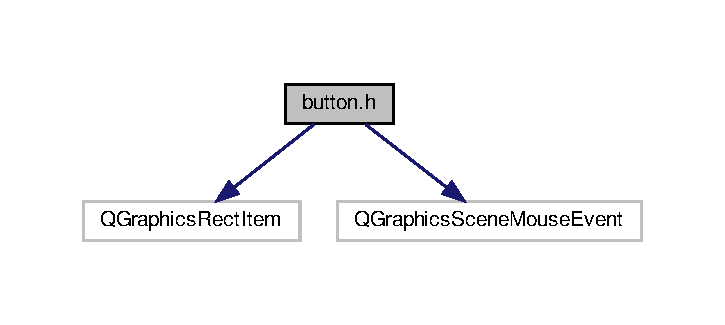
\includegraphics[width=348pt]{button_8h__incl}
\end{center}
\end{figure}
This graph shows which files directly or indirectly include this file\+:
\nopagebreak
\begin{figure}[H]
\begin{center}
\leavevmode
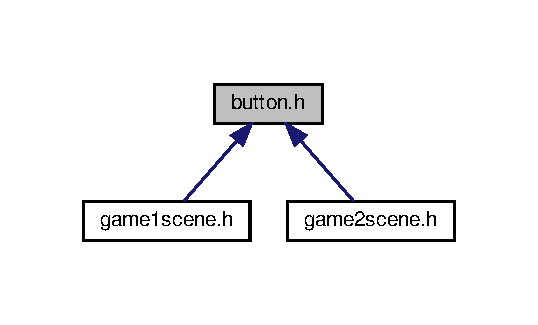
\includegraphics[width=258pt]{button_8h__dep__incl}
\end{center}
\end{figure}
\subsection*{Classes}
\begin{DoxyCompactItemize}
\item 
class \hyperlink{classButton}{Button}
\begin{DoxyCompactList}\small\item\em contains button class definition \end{DoxyCompactList}\end{DoxyCompactItemize}


\subsection{Detailed Description}
contains button class definition 

This class is responsible for creating a button inside a game (QT scene) 
\input{game1menu_8h}
\input{game1scene_8h}
\input{game1score_8h}
\input{game2menu_8h}
\input{game2scene_8h}
\hypertarget{globalvar_8h}{}\section{globalvar.\+h File Reference}
\label{globalvar_8h}\index{globalvar.\+h@{globalvar.\+h}}


contains global variable defintions  


{\ttfamily \#include $<$Q\+String$>$}\newline
{\ttfamily \#include \char`\"{}account.\+h\char`\"{}}\newline
Include dependency graph for globalvar.\+h\+:
\nopagebreak
\begin{figure}[H]
\begin{center}
\leavevmode
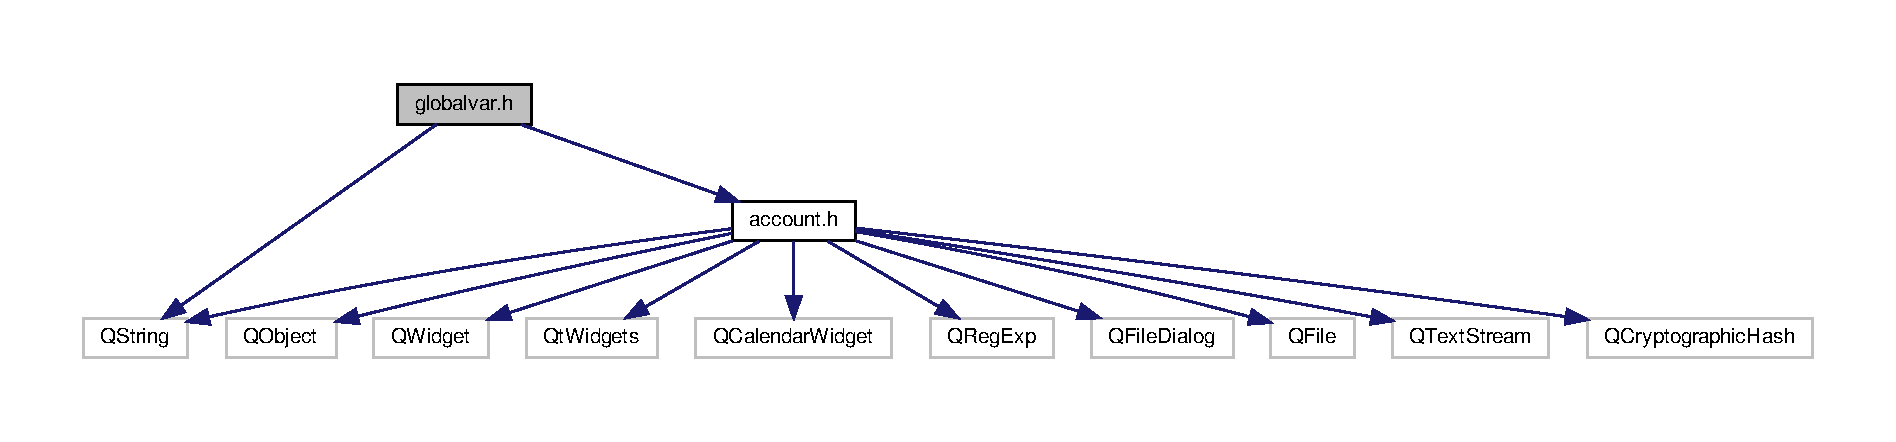
\includegraphics[width=350pt]{globalvar_8h__incl}
\end{center}
\end{figure}
\subsection*{Variables}
\begin{DoxyCompactItemize}
\item 
\mbox{\Hypertarget{globalvar_8h_ac5f844387b3866eed66310b86a47257a}\label{globalvar_8h_ac5f844387b3866eed66310b86a47257a}} 
Q\+String \hyperlink{globalvar_8h_ac5f844387b3866eed66310b86a47257a}{textf}
\begin{DoxyCompactList}\small\item\em string to store textfile path we are using for level choice \end{DoxyCompactList}\item 
\mbox{\Hypertarget{globalvar_8h_a32fb846c339764322967ff655688b373}\label{globalvar_8h_a32fb846c339764322967ff655688b373}} 
Q\+String \hyperlink{globalvar_8h_a32fb846c339764322967ff655688b373}{aud}
\begin{DoxyCompactList}\small\item\em string to store audio file path we are using for level choice \end{DoxyCompactList}\item 
\mbox{\Hypertarget{globalvar_8h_a10c8b97a5a3bbb3eac578d5fc709458e}\label{globalvar_8h_a10c8b97a5a3bbb3eac578d5fc709458e}} 
int \hyperlink{globalvar_8h_a10c8b97a5a3bbb3eac578d5fc709458e}{speedowagon}
\begin{DoxyCompactList}\small\item\em speed for varrying speed for different levels \end{DoxyCompactList}\item 
\mbox{\Hypertarget{globalvar_8h_aa5ceb19e935375a412ac363a2ecf4c1d}\label{globalvar_8h_aa5ceb19e935375a412ac363a2ecf4c1d}} 
\hyperlink{classaccount}{account} $\ast$ \hyperlink{globalvar_8h_aa5ceb19e935375a412ac363a2ecf4c1d}{guest}
\begin{DoxyCompactList}\small\item\em guest account across the whole project \end{DoxyCompactList}\item 
\mbox{\Hypertarget{globalvar_8h_a304a55332026e60c27dda6c3e224b48e}\label{globalvar_8h_a304a55332026e60c27dda6c3e224b48e}} 
bool \hyperlink{globalvar_8h_a304a55332026e60c27dda6c3e224b48e}{turnmasta}
\begin{DoxyCompactList}\small\item\em boolean to determine turn in game 2 \end{DoxyCompactList}\end{DoxyCompactItemize}


\subsection{Detailed Description}
contains global variable defintions 

This file defines global variables used in the project 
\hypertarget{historywidget_8h}{}\section{historywidget.\+h File Reference}
\label{historywidget_8h}\index{historywidget.\+h@{historywidget.\+h}}


contains history widget class defintion  


{\ttfamily \#include $<$Q\+Object$>$}\newline
{\ttfamily \#include $<$Q\+Widget$>$}\newline
{\ttfamily \#include $<$Qt\+Widgets$>$}\newline
{\ttfamily \#include $<$Q\+String$>$}\newline
{\ttfamily \#include $<$Q\+Calendar\+Widget$>$}\newline
{\ttfamily \#include $<$Q\+Reg\+Exp$>$}\newline
{\ttfamily \#include \char`\"{}account.\+h\char`\"{}}\newline
{\ttfamily \#include \char`\"{}game1menu.\+h\char`\"{}}\newline
{\ttfamily \#include $<$Q\+Pixmap$>$}\newline
Include dependency graph for historywidget.\+h\+:\nopagebreak
\begin{figure}[H]
\begin{center}
\leavevmode
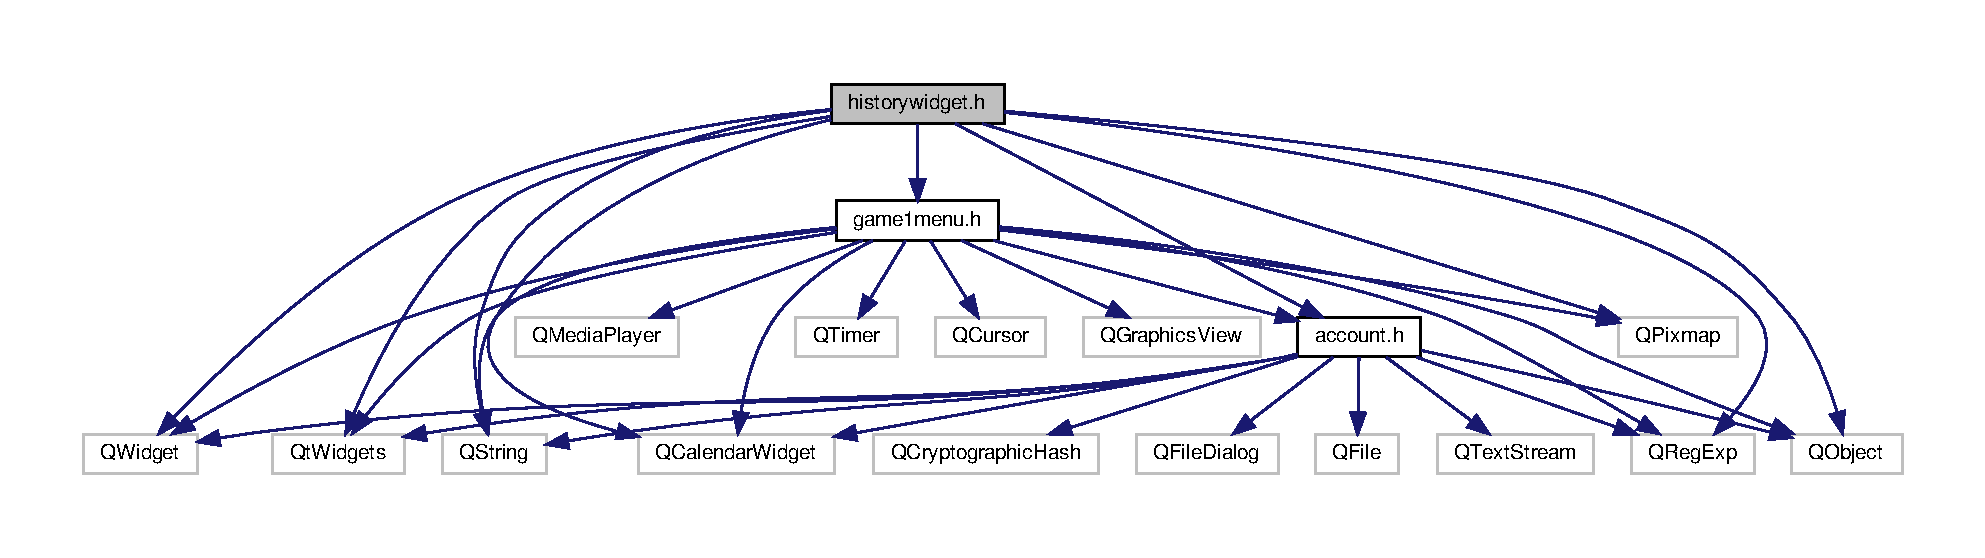
\includegraphics[width=350pt]{historywidget_8h__incl}
\end{center}
\end{figure}
This graph shows which files directly or indirectly include this file\+:\nopagebreak
\begin{figure}[H]
\begin{center}
\leavevmode
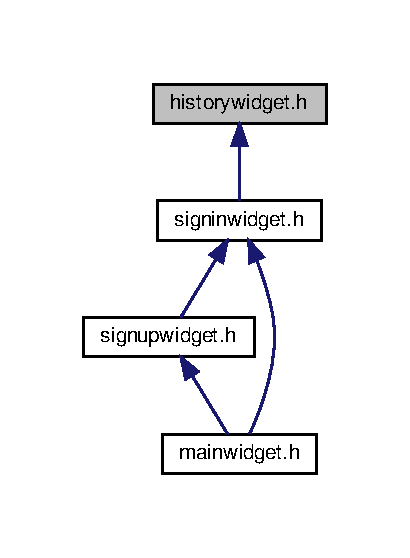
\includegraphics[width=197pt]{historywidget_8h__dep__incl}
\end{center}
\end{figure}
\subsection*{Classes}
\begin{DoxyCompactItemize}
\item 
class \hyperlink{classhistorywidget}{historywidget}
\begin{DoxyCompactList}\small\item\em contains history widget class defintion \end{DoxyCompactList}\end{DoxyCompactItemize}


\subsection{Detailed Description}
contains history widget class defintion 

This class is responsible for constructing the history widget 
\hypertarget{mainwidget_8h}{}\section{mainwidget.\+h File Reference}
\label{mainwidget_8h}\index{mainwidget.\+h@{mainwidget.\+h}}


contains main widget class defintion  


{\ttfamily \#include $<$Q\+Object$>$}\newline
{\ttfamily \#include $<$Q\+Widget$>$}\newline
{\ttfamily \#include $<$Qt\+Widgets$>$}\newline
{\ttfamily \#include $<$Q\+String$>$}\newline
{\ttfamily \#include \char`\"{}signupwidget.\+h\char`\"{}}\newline
{\ttfamily \#include \char`\"{}signinwidget.\+h\char`\"{}}\newline
{\ttfamily \#include \char`\"{}account.\+h\char`\"{}}\newline
{\ttfamily \#include $<$Q\+Cryptographic\+Hash$>$}\newline
Include dependency graph for mainwidget.\+h\+:
\nopagebreak
\begin{figure}[H]
\begin{center}
\leavevmode
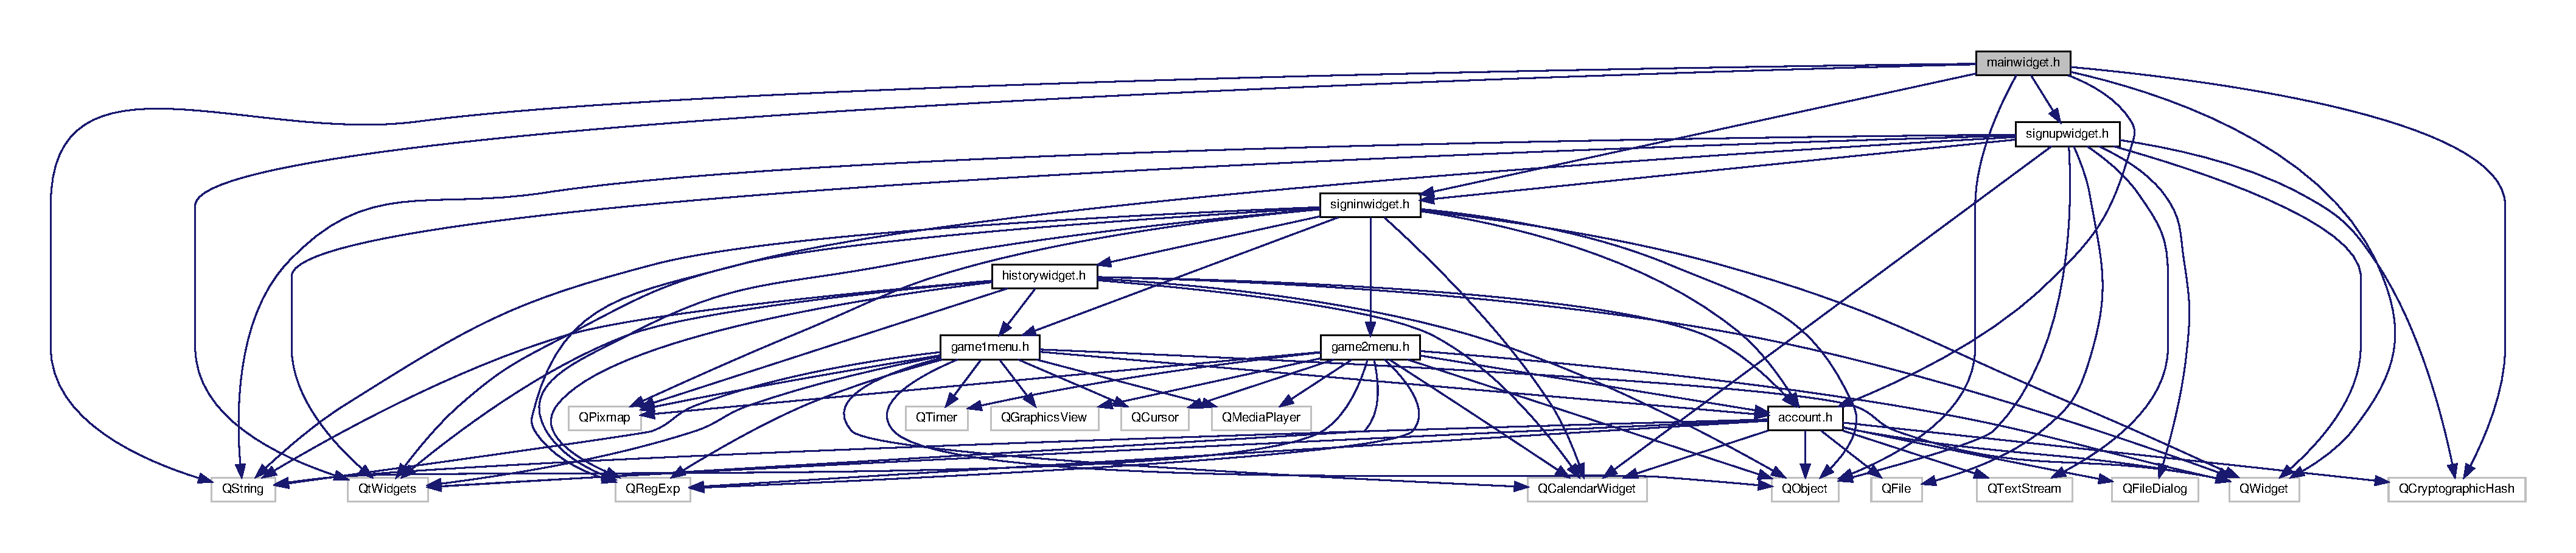
\includegraphics[width=350pt]{mainwidget_8h__incl}
\end{center}
\end{figure}
\subsection*{Classes}
\begin{DoxyCompactItemize}
\item 
class \hyperlink{classmainWidget}{main\+Widget}
\begin{DoxyCompactList}\small\item\em contains main widget class defintion \end{DoxyCompactList}\end{DoxyCompactItemize}


\subsection{Detailed Description}
contains main widget class defintion 

This class is responsible for constructing the main widget 
\input{piece_8h}
\hypertarget{signinwidget_8h}{}\section{signinwidget.\+h File Reference}
\label{signinwidget_8h}\index{signinwidget.\+h@{signinwidget.\+h}}


contains signin widget class defintion  


{\ttfamily \#include $<$Q\+Object$>$}\newline
{\ttfamily \#include $<$Q\+Widget$>$}\newline
{\ttfamily \#include $<$Qt\+Widgets$>$}\newline
{\ttfamily \#include $<$Q\+String$>$}\newline
{\ttfamily \#include $<$Q\+Calendar\+Widget$>$}\newline
{\ttfamily \#include $<$Q\+Reg\+Exp$>$}\newline
{\ttfamily \#include \char`\"{}account.\+h\char`\"{}}\newline
{\ttfamily \#include \char`\"{}game1menu.\+h\char`\"{}}\newline
{\ttfamily \#include \char`\"{}game2menu.\+h\char`\"{}}\newline
{\ttfamily \#include \char`\"{}historywidget.\+h\char`\"{}}\newline
{\ttfamily \#include $<$Q\+Pixmap$>$}\newline
Include dependency graph for signinwidget.\+h\+:\nopagebreak
\begin{figure}[H]
\begin{center}
\leavevmode
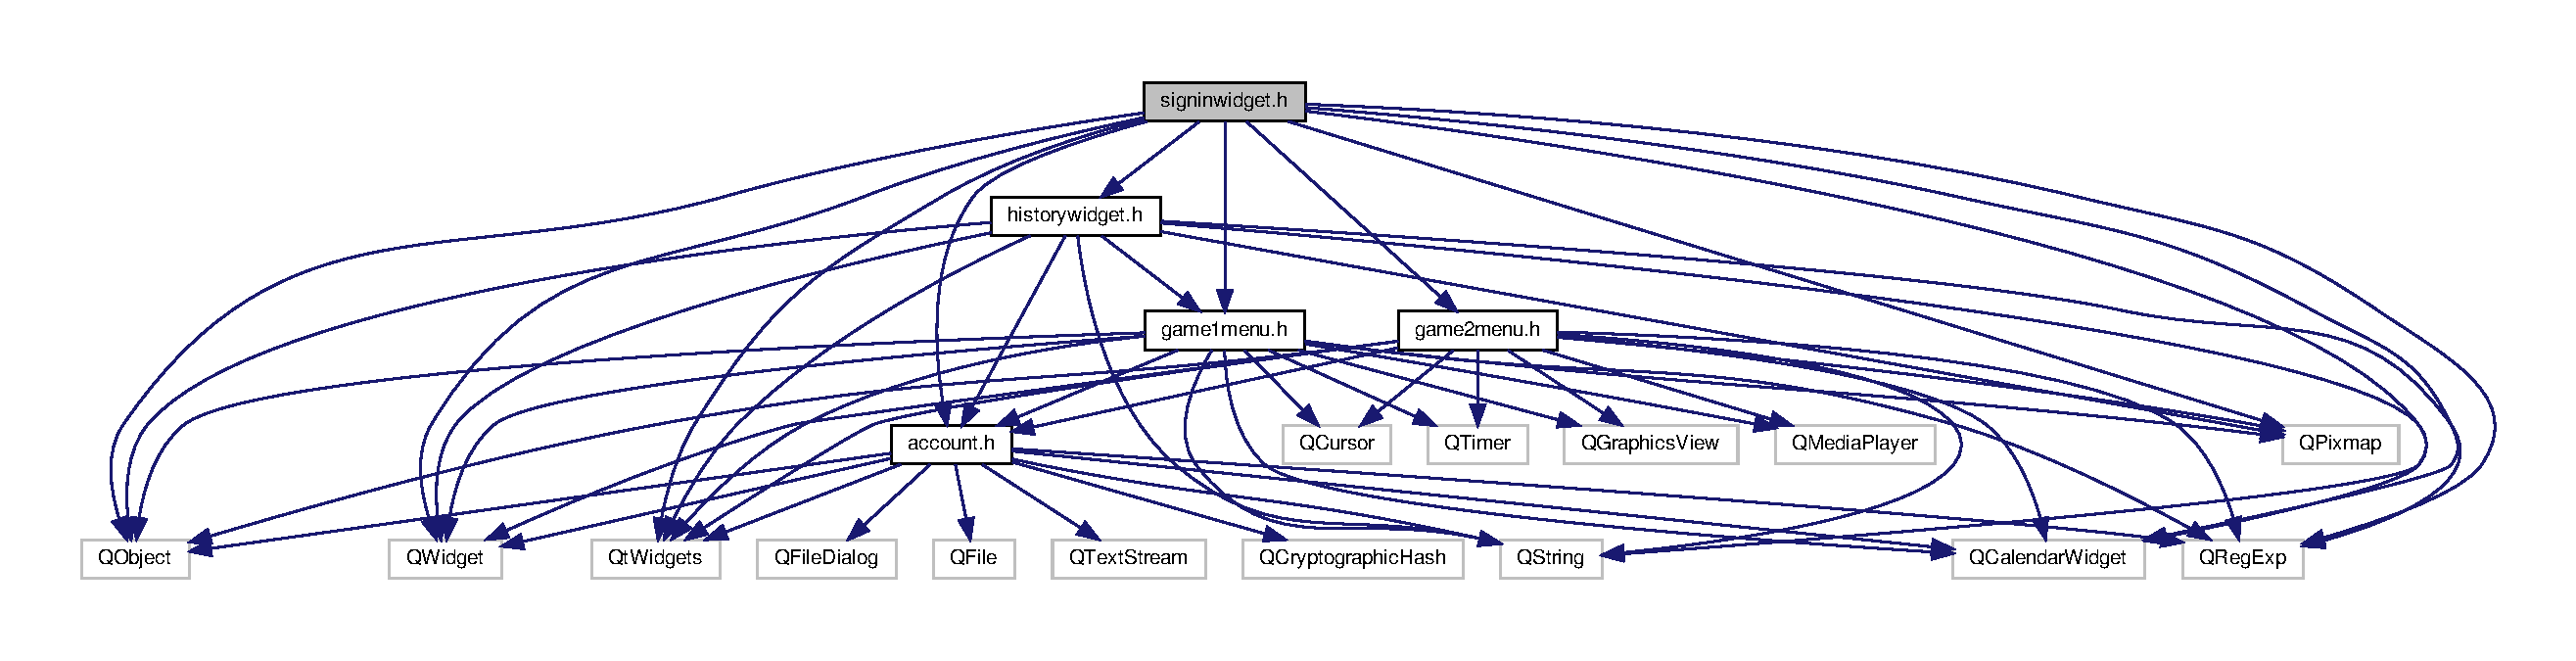
\includegraphics[width=350pt]{signinwidget_8h__incl}
\end{center}
\end{figure}
This graph shows which files directly or indirectly include this file\+:\nopagebreak
\begin{figure}[H]
\begin{center}
\leavevmode
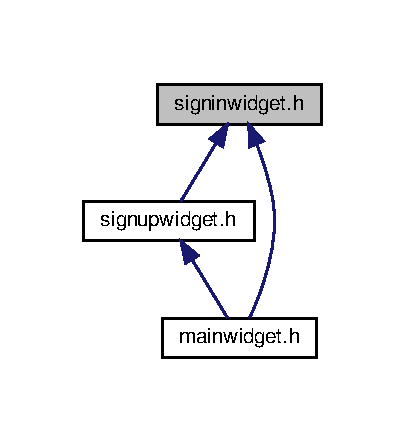
\includegraphics[width=195pt]{signinwidget_8h__dep__incl}
\end{center}
\end{figure}
\subsection*{Classes}
\begin{DoxyCompactItemize}
\item 
class \hyperlink{classsigninwidget}{signinwidget}
\begin{DoxyCompactList}\small\item\em contains signin widget class defintion \end{DoxyCompactList}\end{DoxyCompactItemize}


\subsection{Detailed Description}
contains signin widget class defintion 

This class is responsible for constructing the signin widget 
\hypertarget{signupwidget_8h}{}\section{signupwidget.\+h File Reference}
\label{signupwidget_8h}\index{signupwidget.\+h@{signupwidget.\+h}}


contains signup widget class defintion  


{\ttfamily \#include $<$Q\+Object$>$}\newline
{\ttfamily \#include $<$Q\+Widget$>$}\newline
{\ttfamily \#include $<$Qt\+Widgets$>$}\newline
{\ttfamily \#include $<$Q\+String$>$}\newline
{\ttfamily \#include $<$Q\+Calendar\+Widget$>$}\newline
{\ttfamily \#include $<$Q\+Reg\+Exp$>$}\newline
{\ttfamily \#include $<$Q\+File\+Dialog$>$}\newline
{\ttfamily \#include $<$Q\+File$>$}\newline
{\ttfamily \#include $<$Q\+Text\+Stream$>$}\newline
{\ttfamily \#include $<$Q\+Cryptographic\+Hash$>$}\newline
{\ttfamily \#include \char`\"{}signinwidget.\+h\char`\"{}}\newline
Include dependency graph for signupwidget.\+h\+:\nopagebreak
\begin{figure}[H]
\begin{center}
\leavevmode
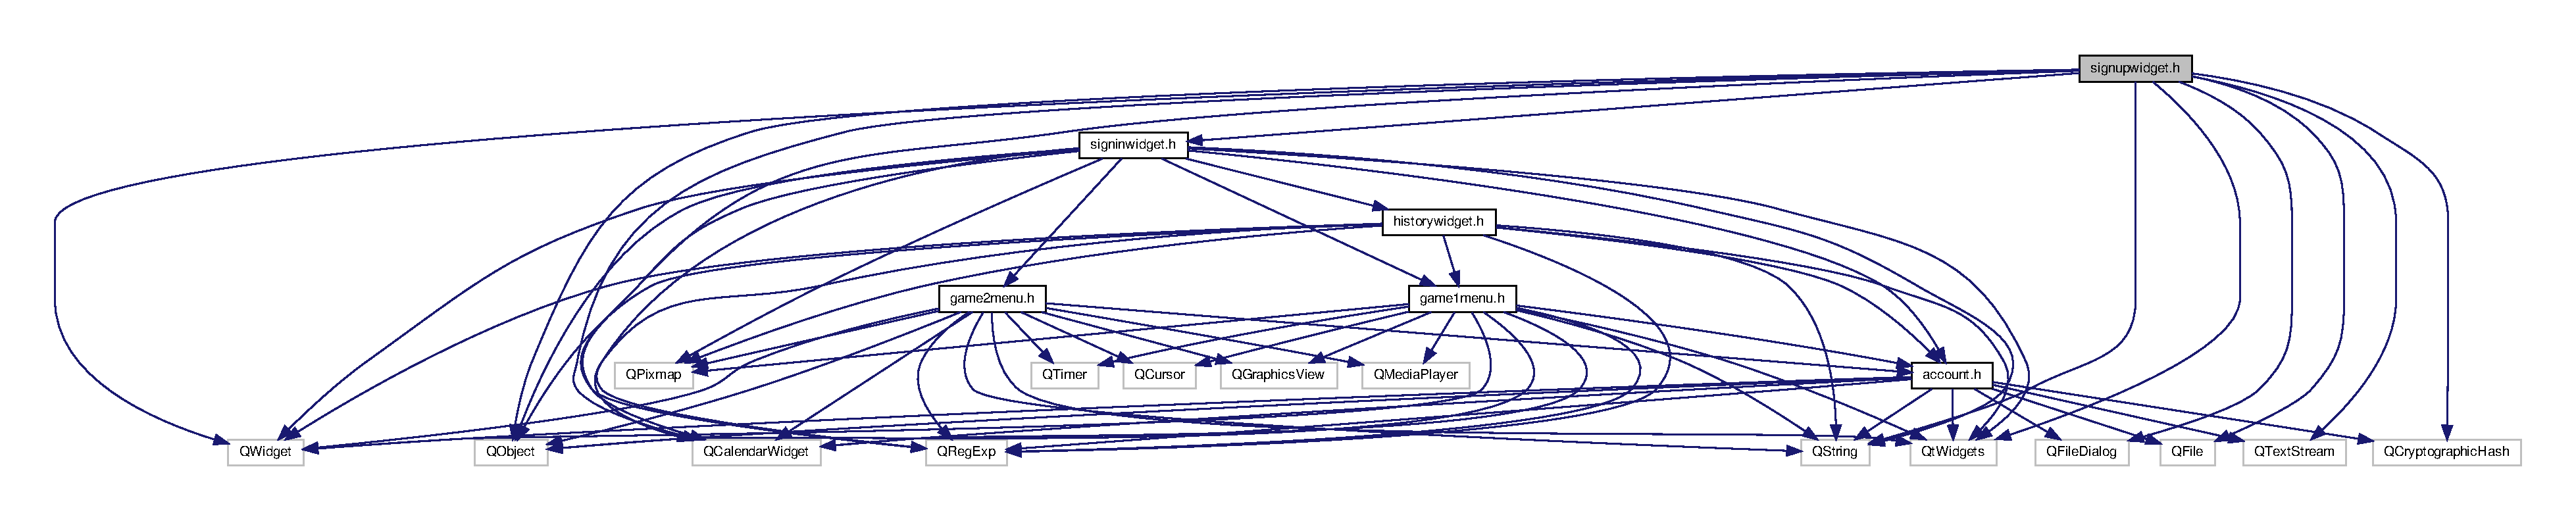
\includegraphics[width=350pt]{signupwidget_8h__incl}
\end{center}
\end{figure}
This graph shows which files directly or indirectly include this file\+:\nopagebreak
\begin{figure}[H]
\begin{center}
\leavevmode
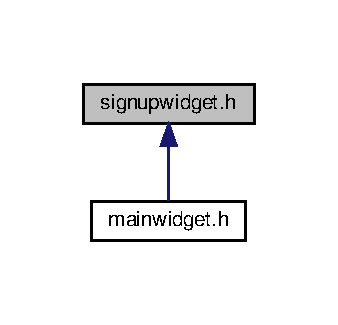
\includegraphics[width=162pt]{signupwidget_8h__dep__incl}
\end{center}
\end{figure}
\subsection*{Classes}
\begin{DoxyCompactItemize}
\item 
class \hyperlink{classsignupwidget}{signupwidget}
\begin{DoxyCompactList}\small\item\em contains signup widget class defintion \end{DoxyCompactList}\end{DoxyCompactItemize}


\subsection{Detailed Description}
contains signup widget class defintion 

This class is responsible for constructing the sign up widget 
\hypertarget{vdeath_8h}{}\section{vdeath.\+h File Reference}
\label{vdeath_8h}\index{vdeath.\+h@{vdeath.\+h}}


contains virus death class definition  


{\ttfamily \#include $<$Q\+Pixmap$>$}\newline
{\ttfamily \#include $<$Q\+Graphics\+Pixmap\+Item$>$}\newline
{\ttfamily \#include $<$Q\+Timer$>$}\newline
{\ttfamily \#include $<$Q\+Graphics\+Scene$>$}\newline
{\ttfamily \#include $<$Q\+Graphics\+Scene\+Mouse\+Event$>$}\newline
Include dependency graph for vdeath.\+h\+:\nopagebreak
\begin{figure}[H]
\begin{center}
\leavevmode
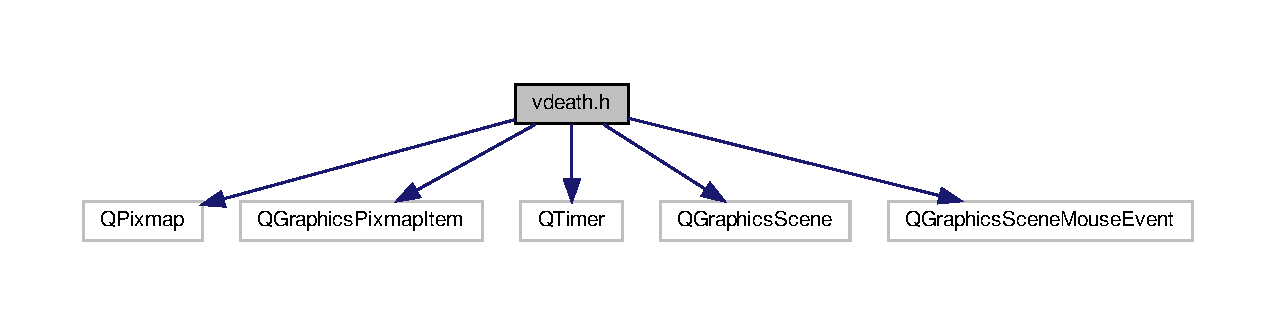
\includegraphics[width=350pt]{vdeath_8h__incl}
\end{center}
\end{figure}
This graph shows which files directly or indirectly include this file\+:\nopagebreak
\begin{figure}[H]
\begin{center}
\leavevmode
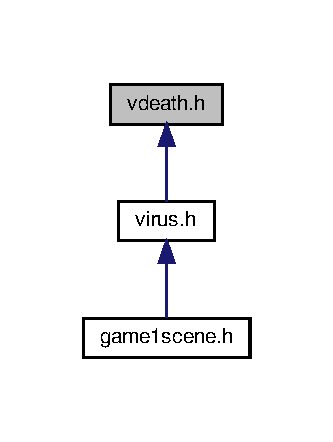
\includegraphics[width=160pt]{vdeath_8h__dep__incl}
\end{center}
\end{figure}
\subsection*{Classes}
\begin{DoxyCompactItemize}
\item 
class \hyperlink{classvdeath}{vdeath}
\begin{DoxyCompactList}\small\item\em contains virus death class definition \end{DoxyCompactList}\end{DoxyCompactItemize}


\subsection{Detailed Description}
contains virus death class definition 

This class is responsible for setting the death animation and removing it from the scene 
\hypertarget{virus_8h}{}\section{virus.\+h File Reference}
\label{virus_8h}\index{virus.\+h@{virus.\+h}}


contains virus class definition definition  


{\ttfamily \#include $<$Q\+Pixmap$>$}\newline
{\ttfamily \#include $<$Q\+Graphics\+Pixmap\+Item$>$}\newline
{\ttfamily \#include $<$Q\+Timer$>$}\newline
{\ttfamily \#include $<$Q\+Graphics\+Scene$>$}\newline
{\ttfamily \#include $<$Q\+Graphics\+Scene\+Mouse\+Event$>$}\newline
{\ttfamily \#include $<$Q\+Media\+Player$>$}\newline
{\ttfamily \#include \char`\"{}vdeath.\+h\char`\"{}}\newline
Include dependency graph for virus.\+h\+:\nopagebreak
\begin{figure}[H]
\begin{center}
\leavevmode
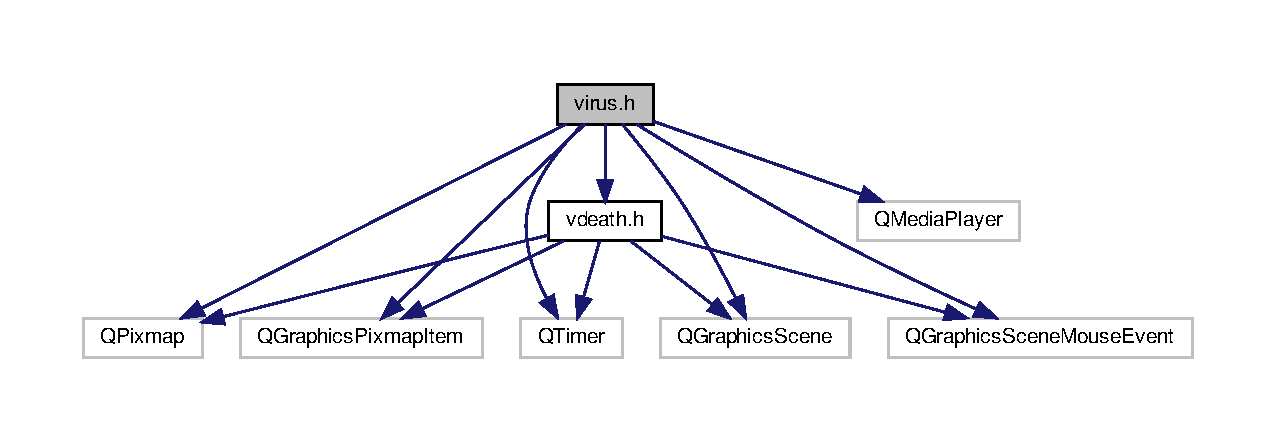
\includegraphics[width=350pt]{virus_8h__incl}
\end{center}
\end{figure}
This graph shows which files directly or indirectly include this file\+:\nopagebreak
\begin{figure}[H]
\begin{center}
\leavevmode
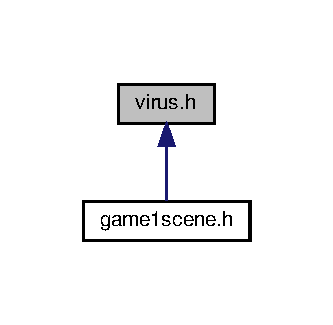
\includegraphics[width=160pt]{virus_8h__dep__incl}
\end{center}
\end{figure}
\subsection*{Classes}
\begin{DoxyCompactItemize}
\item 
class \hyperlink{classvirus}{virus}
\begin{DoxyCompactList}\small\item\em contains virus class definition \end{DoxyCompactList}\end{DoxyCompactItemize}


\subsection{Detailed Description}
contains virus class definition definition 

This class is responsible for creating the viruses for the game along with destroying them on click 
%--- End generated contents ---

% Index
\backmatter
\newpage
\phantomsection
\clearemptydoublepage
\addcontentsline{toc}{chapter}{Index}
\printindex

\end{document}
